\documentclass[12pt, a4paper]{report}
\usepackage[utf8]{inputenc}
\usepackage{mathptmx} % Times New Roman
\usepackage{geometry}
\geometry{a4paper, margin=1in}
\usepackage{setspace}
\setstretch{1.5}
\usepackage{graphicx}
\graphicspath{{figures/}{./}}
\usepackage{titlesec}
\PassOptionsToPackage{hyphens}{url}
\usepackage{hyperref}
\usepackage{fancyhdr}
\usepackage{listings}
\usepackage{xcolor}
\usepackage{tabularx}
\usepackage{booktabs}
\usepackage{longtable}
\usepackage{float}
\usepackage{eso-pic}
\usepackage{tikz}
\usepackage{enumitem}
\usetikzlibrary{calc, shapes.geometric, shapes.multipart, arrows.meta, positioning, fit, backgrounds, decorations.pathreplacing}

% --- PAGE BORDER ---
\definecolor{bordercolor}{HTML}{B3A382} % Khaki/Gold border color matching the Word template
\AddToShipoutPictureBG{%
\begin{tikzpicture}[overlay,remember picture]
\draw[line width=0.5pt, double, double distance=1.5pt, color=bordercolor]
    ($ (current page.north west) + (0.5in,-0.5in) $)
    rectangle
    ($ (current page.south east) + (-0.5in,0.5in) $);
\end{tikzpicture}
}

% --- HEADER & FOOTER ---
\pagestyle{fancy}
\fancyhf{} % Clear defaults
\renewcommand{\headrulewidth}{0pt} % Remove header line
% Set footer for standard pages
\cfoot{\textcolor{blue!60}{\fontsize{9pt}{11pt}\selectfont MIT School of Computing, MIT ADT University}}
\rfoot{\thepage}

% Ensure title pages, certificates, and chapter starting pages also have the footer
\fancypagestyle{empty}{
  \fancyhf{}
  \renewcommand{\headrulewidth}{0pt}
  \cfoot{\textcolor{blue!60}{\fontsize{9pt}{11pt}\selectfont MIT School of Computing, MIT ADT University}}
}
\fancypagestyle{plain}{
  \fancyhf{}
  \renewcommand{\headrulewidth}{0pt}
  \cfoot{\textcolor{blue!60}{\fontsize{9pt}{11pt}\selectfont MIT School of Computing, MIT ADT University}}
  \rfoot{\thepage}
}

% Chapter formatting
\titleformat{\chapter}[display]
  {\normalfont\fontsize{16pt}{19pt}\bfseries\centering}{\chaptertitlename\ \thechapter}{10pt}{\fontsize{16pt}{19pt}\selectfont}
\titlespacing*{\chapter}{0pt}{-20pt}{20pt}
\titleformat{\section}
  {\normalfont\fontsize{14pt}{17pt}\bfseries}{\thesection}{1em}{}
\titleformat{\subsection}
  {\normalfont\fontsize{12pt}{15pt}\bfseries}{\thesubsection}{1em}{}

% Code block styling
\definecolor{codegreen}{rgb}{0,0.6,0}
\definecolor{codegray}{rgb}{0.5,0.5,0.5}
\definecolor{codepurple}{rgb}{0.58,0,0.82}
\definecolor{backcolour}{rgb}{0.95,0.95,0.92}
\definecolor{mitpurple}{HTML}{7030A0} % Deep purple matching Word

\lstdefinestyle{mystyle}{
    backgroundcolor=\color{backcolour},   
    commentstyle=\color{codegreen},
    keywordstyle=\color{blue},
    numberstyle=\tiny\color{codegray},
    stringstyle=\color{codepurple},
    basicstyle=\ttfamily\small,
    breakatwhitespace=false,         
    breaklines=true,                 
    captionpos=b,                    
    keepspaces=true,                 
    numbers=left,                    
    numbersep=5pt,                  
    showspaces=false,                
    showstringspaces=false,
    showtabs=false,                  
    tabsize=2
}
\lstset{style=mystyle}

% Colors for TikZ
\definecolor{primary}{RGB}{225,29,72}
\definecolor{secondary}{RGB}{13,148,136}
\definecolor{accent}{RGB}{245,158,11}
\definecolor{dark}{RGB}{15,23,42}
\definecolor{lightgray}{RGB}{241,245,249}
\definecolor{midgray}{RGB}{148,163,184}
\definecolor{success}{RGB}{16,185,129}
\definecolor{danger}{RGB}{239,68,68}
\definecolor{tablebg}{HTML}{f8fafc}
\definecolor{tableborder}{HTML}{cbd5e1}

\begin{document}
\pagenumbering{roman}

% --- TITLE PAGE ---
\begin{titlepage}
    \centering
    \vspace*{0.5cm}
    
    {\Large \textbf{A JURY PROJECT REPORT}}\\[0.3cm]
    \textit{Submitted in partial fulfillment of the requirements} \\
    \textit{for the award of the degree of}\\[0.3cm]
    
    {\Large \textbf{BACHELOR OF TECHNOLOGY}} \\
    \textit{in} \\
    {\large \textbf{COMPUTER SCIENCE \& ENGINEERING}}\\[0.3cm]
    
    \textcolor{mitpurple}{\textbf{SUBJECT: DATA WAREHOUSING AND DATA MINING (DWDM)}}\\[0.3cm]
    \textcolor{mitpurple}{\textbf{JURY II: UNITS III \& IV}}\\[0.8cm]
    
    {\LARGE \textbf{``Customer Behavioral Analysis and\\[0.2cm] Loan Default Classification''}}\\[0.35cm]
    {\large \textit{A Data Mining Approach to Credit Risk on the PKDD'99 Dataset}}\\[0.8cm]
    
    \textbf{SUBMITTED BY:}\\
    Dhanush Pillay \hspace{1cm} ADT24SOCB0765 \\
    Shubhangini Dixit \hspace{0.65cm} ADT24SOCB1156 \\
    Semester: $5^{th}$ Semester / TY BDCE \\[0.5cm]
    
    \textbf{INTERNAL FACULTY GUIDE:}\\
    Dr. Reena Pagare \\
    Department of Computer Science \& Engineering \\[0.5cm]
    
    \vfill
    
    \textbf{DEPARTMENT OF COMPUTER SCIENCE \& ENGINEERING}\\
    \textcolor{mitpurple}{\textbf{MIT ART, DESIGN AND TECHNOLOGY UNIVERSITY, PUNE}}\\
    Loni Kalbhor, Pune, MH, India -- 412201
\end{titlepage}




\newpage
\begin{spacing}{1.35}
\tableofcontents
\end{spacing}
\listoffigures
\listoftables

\clearpage
\pagenumbering{arabic}

\chapter{Introduction}

\section{Problem Definition}
Banking institutions sit on large volumes of operational data: account histories, transactions, demographics, and loan records. The information that predicts whether a borrower will repay a loan is usually already present in that history before the loan is granted, but it is buried in millions of individual transactions and is not directly usable by a credit officer.

This project addresses the resulting decision problem as a supervised binary classification task. Given a loan application and the applicant's pre-loan transaction history, the system estimates whether the loan will be repaid (a \emph{good} loan) or will default (a \emph{bad} loan). The task is performed on the PKDD'99 Financial Dataset, which contains 682 loans and roughly one million account transactions from a Czech bank between 1993 and 1998. Of the 682 loans, 606 were repaid and 76 defaulted, giving a base default rate of 11.14 percent.

The central constraint is temporal: every behavioral feature is computed only from transactions dated strictly before the loan grant date. Post-loan activity is never used, so the model reproduces what the bank could have known at decision time rather than what it learned afterwards.

\section{Motivation and Business Context}
Loan defaults are direct losses, while rejected good customers are opportunity costs. A model that separates the two groups well allows the bank to route applications into a review queue, ask for additional collateral, or adjust the offered amount. The cost of the two error types is not symmetric: approving a future defaulter is usually more expensive than reviewing a good customer twice.

The dataset is also strongly imbalanced. With only 11.14 percent positives, a trivial classifier that predicts ``repaid'' for every application reaches 88.86 percent accuracy while catching zero defaulters. Accuracy is therefore not a useful headline metric here, and the evaluation has to focus on the positive class: precision, recall, F1-score, Average Precision, and ROC-AUC. This project treats that methodological point as part of the problem, not as an afterthought.

\section{Project Objectives}
The project covers the complete data mining pipeline required by Units III and IV of the syllabus. Its objectives are:

\begin{enumerate}
    \item To clean and integrate the raw PKDD'99 tables into a single loan-level analytical dataset.
    \item To engineer behavioral features from pre-loan transactions only, and to verify that no post-loan information leaks into the feature set.
    \item To perform exploratory data analysis and visualize the behavioral differences between repaid and defaulted loans.
    \item To train and compare six classification algorithms: Decision Tree, Naive Bayes, Random Forest, Support Vector Machine (SVM), K-Nearest Neighbors (KNN), and Gradient Boosting.
    \item To handle class imbalance explicitly by training each classifier twice, once on the raw data and once on a SMOTE-balanced training set.
    \item To tune hyperparameters and select the final model using repeated stratified cross-validation rather than a single train--test split.
    \item To interpret the selected model through feature importance and association rule mining, and to translate the findings into business recommendations.
\end{enumerate}

\section{Scope and Deliverables}
The project scope is limited to binary loan-default classification on historical data. It does not include live scoring, credit-policy design, or causal analysis. The supplementary components are customer segmentation with KMeans, association rule mining with Apriori and FP-Growth, and a Streamlit decision-support console that reads the exported result files.

Table~\ref{tab:deliverables} maps each expected deliverable to the artifact that implements it.

\begin{table}[H]
    \centering
    \small
    \renewcommand{\arraystretch}{1.25}
    \begin{tabularx}{\textwidth}{|>{\raggedright\arraybackslash}p{4.6cm}|>{\raggedright\arraybackslash}X|}
        \hline
        \textbf{Deliverable} & \textbf{Where it is implemented} \\
        \hline
        Problem definition and objectives & This chapter and \texttt{docs/Problem\_Statement.md} \\
        \hline
        Dataset description and source & Chapter 2; raw CSVs in \texttt{data/} \\
        \hline
        Data preprocessing pipeline & Chapter 4; \texttt{01\_preprocessing.ipynb}, \texttt{02\_features.ipynb} \\
        \hline
        EDA and visualizations & Chapter 5; \texttt{03\_eda.ipynb}; 8 EDA figures, 14 project figures in total \\
        \hline
        Classification algorithms & Chapter 6; \texttt{04\_modeling.ipynb} \\
        \hline
        Performance comparison & Chapter 6; \texttt{metrics\_comparison.csv}, \texttt{tuning\_results.csv}, \texttt{cv\_comparison.csv} \\
        \hline
        Conclusions and recommendations & Chapter 7; \texttt{docs/Jury2\_Report.md} \\
        \hline
        Association rule mining (Unit III) & Section 6.8; \texttt{tools/pattern\_mining.py} \\
        \hline
        Project report and presentation & This document and the executed notebooks \\
        \hline
    \end{tabularx}
    \caption{Deliverable coverage for Jury II}
    \label{tab:deliverables}
\end{table}

\section{Jury II Evaluation Coverage}
\label{sec:evaluation-coverage}

Table~\ref{tab:jury2-coverage} maps the evaluation parameters for Jury II to the parts of this report that address them. The table is an index, not a substitute for the chapters: each row points to the analysis, table, or figure that contains the evidence.

\begin{table}[htbp]
    \centering
    \small
    \renewcommand{\arraystretch}{1.2}
    \begin{tabularx}{\textwidth}{@{}>{\raggedright\arraybackslash}p{4.4cm}X@{}}
        \toprule
        \textbf{Evaluation parameter} & \textbf{Coverage in this report} \\
        \midrule
        Dataset & Chapter~\ref{ch:literature}, Table~\ref{tab:pkdd_tables}; source joins and cleaning in Chapter~\ref{ch:preprocessing}. \\
        \addlinespace
        Architecture diagram & Figure~\ref{fig:architecture} and the stage description in Section~\ref{sec:pipeline-stages}. \\
        \addlinespace
        Input / output & Section~\ref{sec:io}, Table~\ref{tab:io}; the 18-feature model input and scored output are stated there. \\
        \addlinespace
        Classes / labels & Section~\ref{sec:target-definition}, Table~\ref{tab:target-balance}; the A/C versus B/D mapping and the 606/76 balance. \\
        \addlinespace
        Pattern matching (FP-Growth, Apriori) & Section~\ref{sec:pattern-mining}, Table~\ref{tab:pattern-rules}; both algorithms, the 41 itemsets, and the two default rules. \\
        \addlinespace
        Comparison with other classification algorithms & Sections~\ref{sec:test-results} and~\ref{sec:cv-results}, Tables~\ref{tab:test-results} and~\ref{tab:cv-results}; six classifiers under baseline and SMOTE. \\
        \addlinespace
        Classification algorithm & Chapter~\ref{ch:literature} and Sections~\ref{sec:classifiers} and~\ref{sec:training-pipeline}; the six learners and their pipelines. \\
        \addlinespace
        Innovation added to the classification algorithm & Section~\ref{sec:innovation}; the pre-loan representation, balance-capacity view, two-arm validation, and rule-plus-model review layer. \\
        \addlinespace
        Performance metrics & Section~\ref{sec:evaluation-protocol} and Sections~\ref{sec:test-results} and~\ref{sec:ranking-curves}; accuracy, precision, recall, F1, AP, ROC-AUC, and confusion matrices. \\
        \addlinespace
        Chart & Chapter~\ref{ch:eda} and Figures~\ref{fig:roc-curves} and~\ref{fig:pr-curves}; the Streamlit console in Section~\ref{sec:streamlit} presents the same charts. \\
        \bottomrule
    \end{tabularx}
    \caption{Coverage of the Jury II evaluation parameters.}
    \label{tab:jury2-coverage}
\end{table}

\section{Organization of the Report}
Chapter 2 reviews the dataset, the classifiers, imbalance handling, and the evaluation metrics. Chapter 3 describes the system architecture, the input and output specification, leakage controls, and the evaluation protocol. Chapter 4 documents data cleaning and feature engineering. Chapter 5 presents the exploratory analysis. Chapter 6 reports the model implementation, tuning, comparison, feature importance, and pattern mining. Chapter 7 states the conclusions, innovation, limitations, and future scope. Section~\ref{sec:evaluation-coverage} maps each Jury II evaluation parameter to these chapters.

\chapter{Literature Review and Background}
\label{ch:literature}

\section{The PKDD'99 Financial Dataset}
\label{sec:dataset}
This project uses the \textbf{PKDD'99 Financial Dataset}, also known as the Berka Dataset, released for the Discovery Challenge at the 1999 European Conference on Principles and Practice of Knowledge Discovery in Databases. It contains anonymized real-world records from a Czech bank covering 1993 to 1998.

The raw data is highly normalized and spread across eight tables. Five are used here. Table~\ref{tab:pkdd_tables} summarizes them.

\begin{table}[H]
    \centering
    \small
    \renewcommand{\arraystretch}{1.25}
    \begin{tabularx}{\textwidth}{|l|r|>{\raggedright\arraybackslash}X|}
        \hline
        \textbf{Table} & \textbf{Rows} & \textbf{Role in this project} \\
        \hline
        \texttt{loan.csv} & 682 & One row per granted loan: account, grant date, amount, duration, installment, and status code. Source of the target. \\
        \hline
        \texttt{trans.csv} & 1,056,320 & One row per account transaction, 1993-01-01 to 1998-12-31. Source of all behavioral features. \\
        \hline
        \texttt{client.csv} & 5,369 & Client identifier, birth number (encodes date of birth and gender), and district. Source of age and gender. \\
        \hline
        \texttt{account.csv} & 4,500 & Account identifier, district, statement frequency, and creation date. Used for provenance. \\
        \hline
        \texttt{disp.csv} & 5,369 & Links clients to accounts as OWNER or DISPONENT. Only OWNER links are used, so every loan maps to one client. \\
        \hline
    \end{tabularx}
    \caption{PKDD'99 tables used in the project}
    \label{tab:pkdd_tables}
\end{table}

The dataset is a standard benchmark for relational data mining because it combines long transaction histories with a small, well-defined loan outcome. This project reads the raw CSV extracts directly. No warehouse, BI tool, or external database is part of the pipeline.

\section{Classification Algorithms}
Six supervised learners are compared. They were chosen to cover different inductive biases rather than to maximize the leaderboard.

\subsection{Decision Tree}
A decision tree partitions the feature space with axis-aligned splits chosen to reduce impurity. It captures non-linear interactions, is easy to explain, and serves as an interpretable baseline. Its main weakness is variance: small changes in the training data can change the tree structure. The search in this project tunes maximum depth, minimum samples per leaf, and the splitting criterion.

\subsection{Naive Bayes}
Gaussian Naive Bayes models each feature as a normal distribution conditional on the class and assumes conditional independence. It is fast and needs very little data, but the independence assumption is clearly violated here because balance and volume features are correlated. It is included as a probabilistic baseline, not as a candidate for deployment.

\subsection{Random Forest}
Random Forest [9] averages many decorrelated decision trees, each grown on a bootstrap sample with a random subset of features at every split. The averaging reduces variance and the out-of-bag behaviour gives a stable impurity-based importance ranking. It is typically strong on small tabular problems and is the reference model for feature importance in this report.

\subsection{Support Vector Machine}
An SVM finds a maximum-margin separating hyperplane, using the kernel trick to represent non-linear boundaries. With 682 rows and 18 features it is computationally comfortable. Because the ROC and precision--recall curves need probability estimates, the SVM is wrapped in \texttt{CalibratedClassifierCV} with a sigmoid calibration and cross-validated calibration folds.

\subsection{K-Nearest Neighbors}
KNN classifies a point by the majority label among its $k$ nearest training neighbours. It makes no global assumption about the decision boundary and provides a distance-based sanity check. It is sensitive to feature scaling, which is why the scaler is part of the pipeline, and it usually struggles when the positive class is rare.

\subsection{Gradient Boosting}
Gradient Boosting [10] fits shallow trees sequentially, each new tree correcting the residual errors of the current ensemble. With a low learning rate and subsampling it often outperforms a single tree and a random forest on structured tabular data. The search tunes the number of estimators, depth, learning rate, and subsample fraction.

\section{Class Imbalance and SMOTE}
The target is imbalanced at roughly 9:1. A classifier optimized for accuracy will usually predict the majority class and ignore defaulters. Two responses are common: cost-sensitive learning and resampling. This project uses SMOTE [8] as the resampling arm, because it is the standard oversampling method and is easy to place inside a scikit-learn pipeline.

SMOTE generates synthetic minority examples by interpolating between a minority point and its nearest minority neighbours. It increases the minority region rather than duplicating points, which reduces the risk of exact overfitting. The comparison in this report is deliberately two-armed: every classifier is trained once on the raw training data and once on a SMOTE-balanced copy, with all resampling fitted inside the training fold only. As Chapter 6 shows, the balanced arm does not help the stronger models, a result that only repeated validation made visible.

\section{Evaluation Metrics under Imbalance}
Accuracy is reported but never used for selection. The primary metrics are:

\begin{itemize}
    \item \textbf{Precision:} of the loans flagged as default, the fraction that actually defaulted.
    \item \textbf{Recall:} of the loans that actually defaulted, the fraction that were flagged.
    \item \textbf{F1-score:} the harmonic mean of precision and recall, used as the selection criterion.
    \item \textbf{Average Precision (AP):} the area under the precision--recall curve, which summarizes ranking quality for the positive class.
    \item \textbf{ROC-AUC:} the probability that a random defaulter is ranked above a random repayer.
\end{itemize}

ROC-AUC can look flattering when the positive class is rare, because a large number of true negatives inflates the false-positive-rate denominator. Average Precision does not have that property, so both are reported. The comparison also uses a confusion matrix per configuration so that the trade-off between missed defaults and false alarms stays visible.

\section{Model Selection and Cross-Validation}
A single 75/25 split leaves about 19 defaults in the test set. At that size, the ranking of twelve configurations is dominated by split noise. The project therefore separates three questions: a readable held-out table at default hyperparameters, a hyperparameter search on the training split, and a repeated stratified cross-validation over all configurations. The final choice uses the repeated 5-fold $\times$ 10 protocol, which yields 50 estimates per configuration and makes the fold-to-fold spread explicit. This follows the standard CRISP-DM emphasis on evaluation as an iterative, evidence-based stage rather than a single number [11].

\section{Related Work and Positioning}
The Berka dataset has been used for loan-default prediction, customer segmentation, and relational feature construction. Much of the published work either uses post-loan information, which is unavailable at decision time, or reports a single train--test split on a small positive class. This project is positioned differently in three ways: the feature set is strictly pre-loan, the comparison includes a balanced and an unbalanced arm for every model, and model selection rests on repeated cross-validation with the uncertainty reported. The association rule mining step is included as a descriptive complement, not as a competitor to the classifiers.

% Chapter 3
\chapter{System Architecture and Methodology}
\label{ch:methodology}

This chapter describes how the project turns five raw PKDD'99 tables into a scored loan portfolio. The work is organised as an offline analytical pipeline with four layers: data assembly, feature engineering, modelling, and serving. Each layer writes a durable artifact, so a result shown in the report or the dashboard can be traced back to a file produced by an earlier stage.

\section{Pipeline Overview}
\label{sec:pipeline-overview}

Figure~\ref{fig:architecture} shows the end-to-end flow. The data layer reads the loan, transaction, client, account, and disposition tables. The feature layer builds one row per loan using only transactions dated before the loan was granted. The modelling layer trains six classifiers under two imbalance settings, tunes them, and evaluates them with a held-out split and repeated cross-validation. The serving layer exposes the resulting metrics, feature importances, risk scores, and mined patterns through a Streamlit console.

\begin{figure}[H]
    \centering
    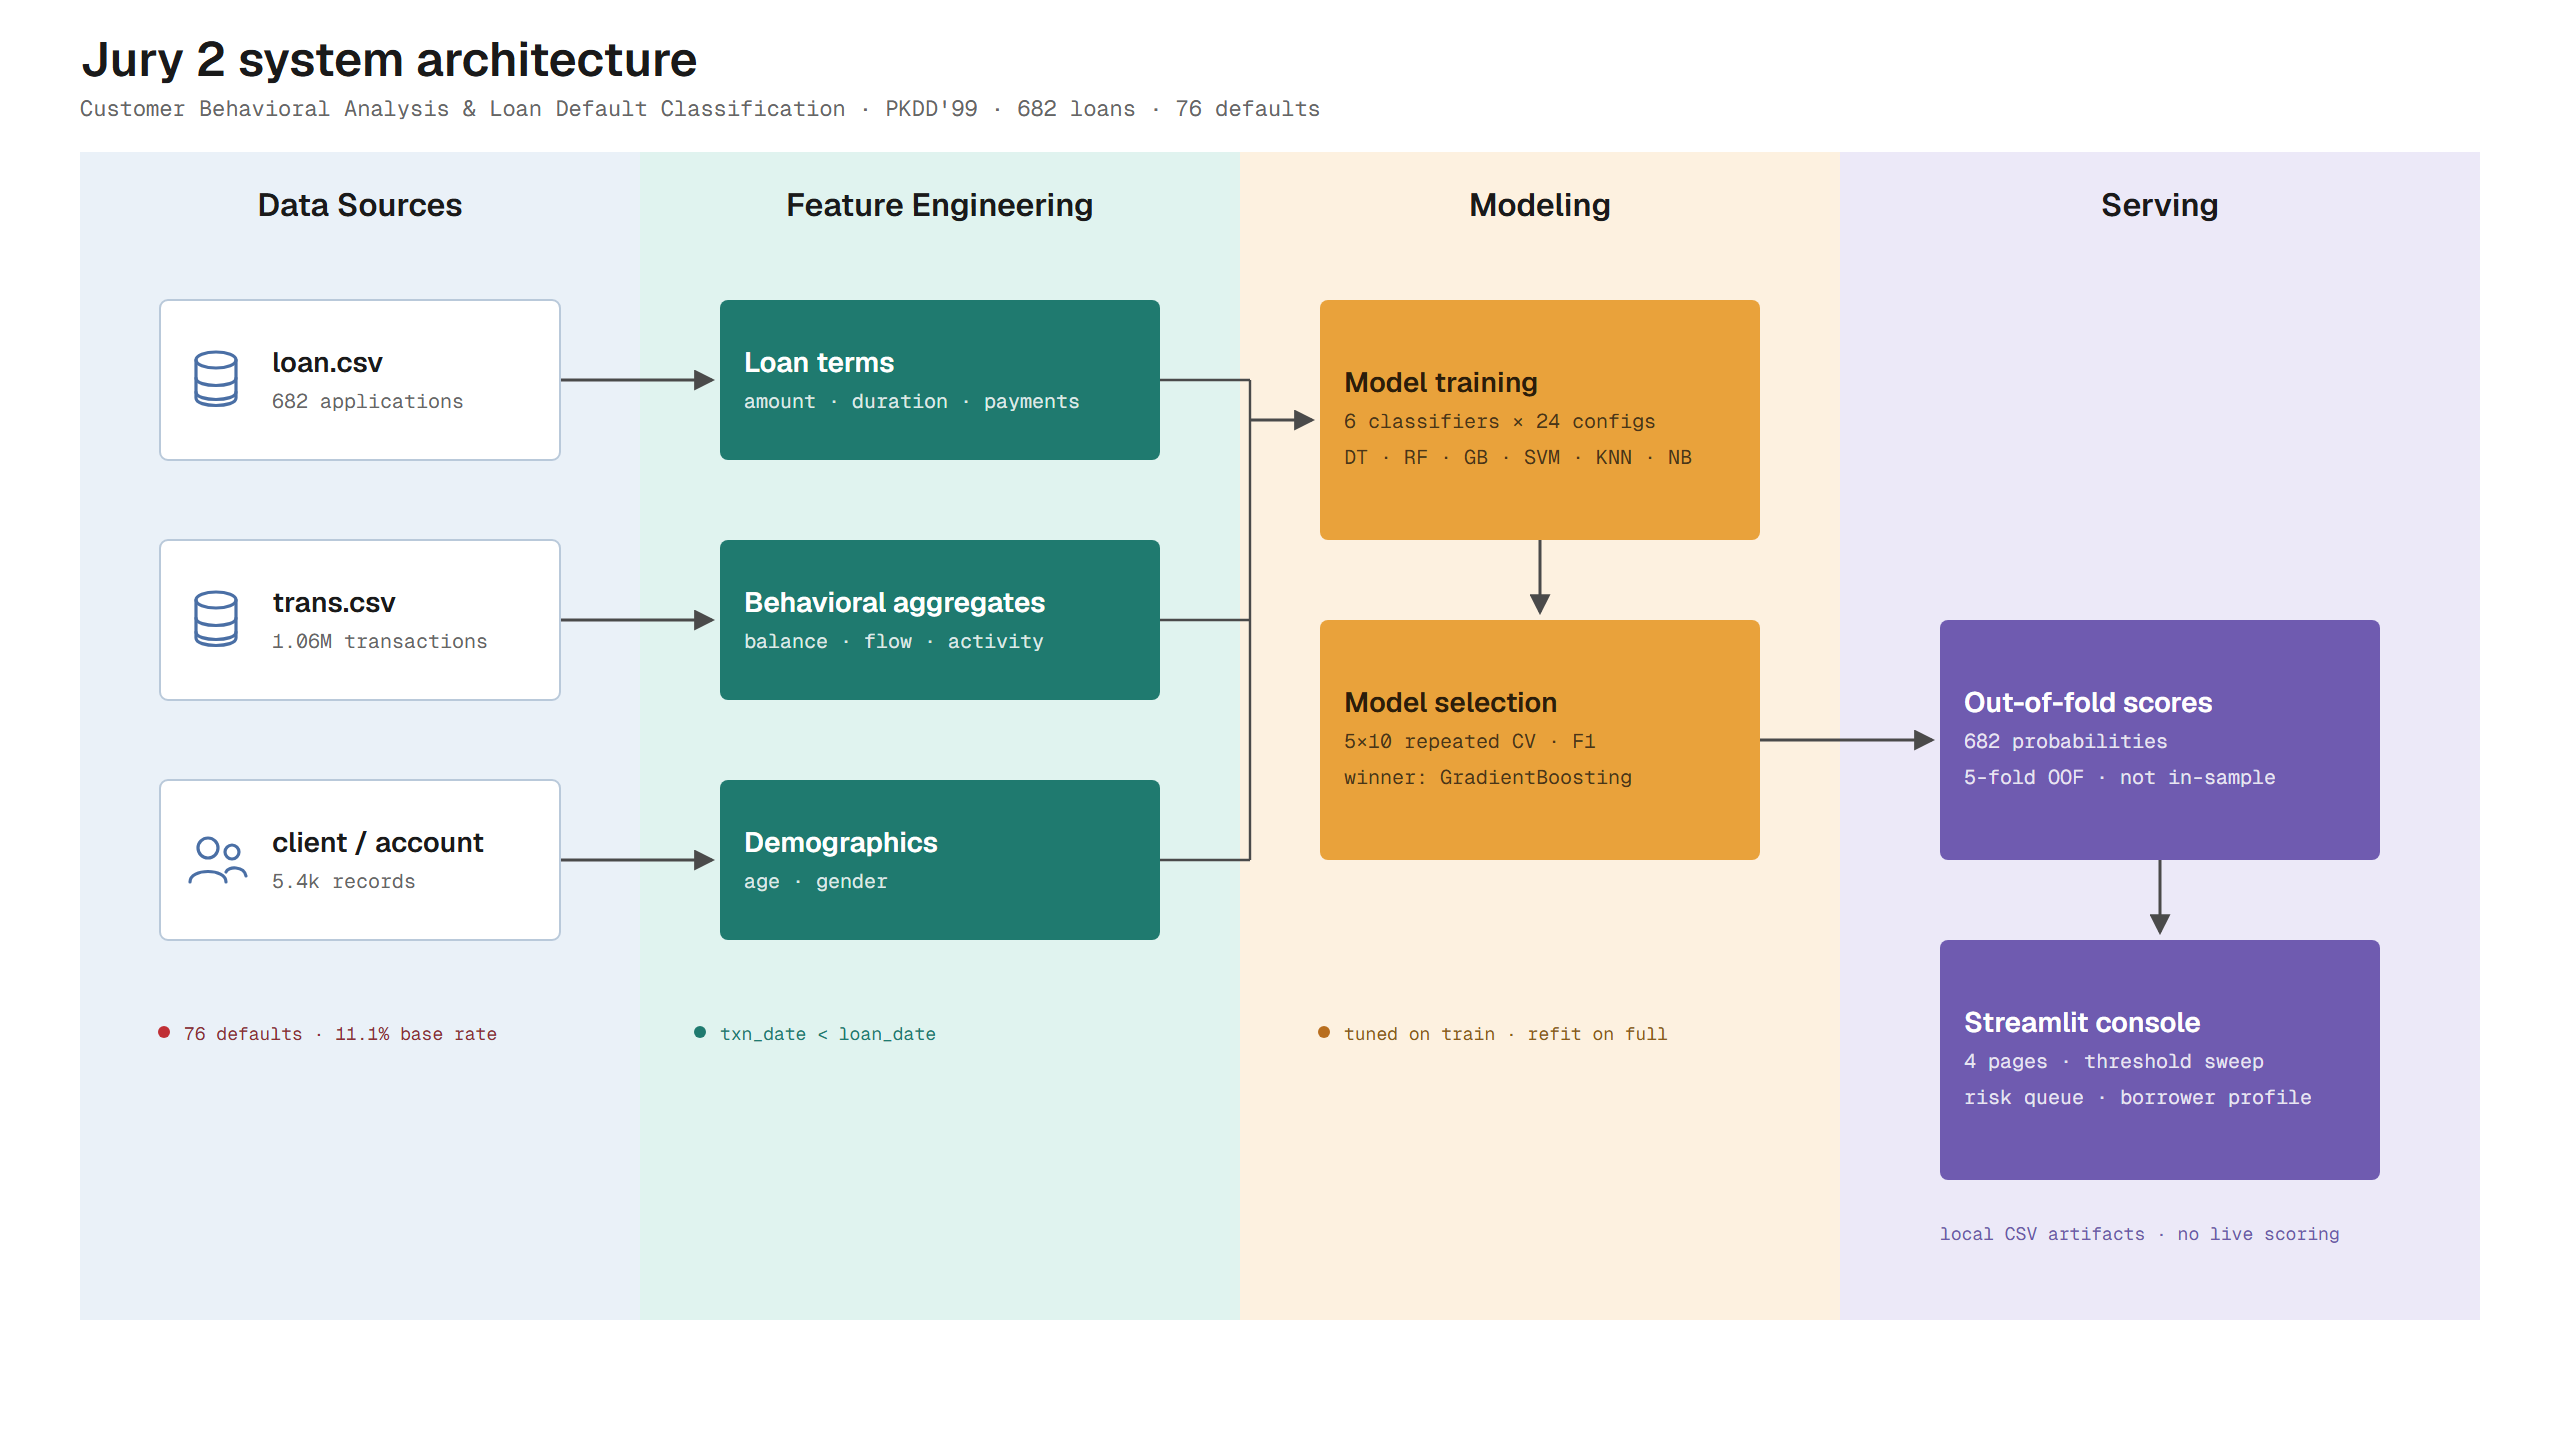
\includegraphics[width=\textwidth]{jury2-architecture.png}
    \caption{End-to-end architecture of the loan default classification project. The pipeline is batch-oriented: each stage reads files from the previous stage and writes a versioned artifact.}
    \label{fig:architecture}
\end{figure}

The design keeps the analytical work separate from the presentation work. Notebooks produce CSV and PNG artifacts under \texttt{outputs/}; the dashboard only reads those artifacts and does not retrain a model when a page is opened. This makes the reported numbers stable and allows the console to run on a machine without the full training environment.

\section{Technology Stack}
\label{sec:technology-stack}

The implementation uses open-source Python tools. Table~\ref{tab:stack} lists the main components and their responsibilities.

\begin{table}[H]
    \centering
    \caption{Tools used in the project and their roles.}
    \label{tab:stack}
    \begin{tabularx}{\textwidth}{@{}lX@{}}
        \toprule
        \textbf{Tool} & \textbf{Role in the project} \\
        \midrule
        Python 3.13.5 & Main programming language for all notebooks and scripts. \\
        pandas 2.2.3 & Reading the CSV extracts, joining tables, and building loan-level features. \\
        NumPy 2.2.4 & Numeric operations and array handling inside pandas and scikit-learn. \\
        scikit-learn 1.7.0 & Classifiers, pipelines, scaling, cross-validation, and hyperparameter search. \\
        imbalanced-learn 0.14.2 & SMOTE oversampling inside the modelling pipeline. \\
        matplotlib 3.10.3 & Base plotting for the figures in this report. \\
        seaborn 0.13.2 & Distribution, box, and correlation plots. \\
        mlxtend & Apriori and FP-Growth pattern mining. \\
        Jupyter Notebook & Literate analysis; notebooks are executed in order with nbconvert. \\
        Streamlit & Interactive review console for the exported results. \\
        \bottomrule
    \end{tabularx}
\end{table}

The versions shown for the core Python libraries are the ones recorded for the analysis environment. The notebooks also rely on the standard library modules \texttt{pathlib}, \texttt{json}, and \texttt{warnings}. No database server or distributed compute engine is required; the largest table, \texttt{trans.csv}, has 1,056,320 rows and fits comfortably in memory on a laptop.

\section{Pipeline Stages}
\label{sec:pipeline-stages}

\subsection{Data Assembly}
The five source files are loaded with explicit column types where needed. The disposition table links clients to accounts. A client can be an owner or a disbursent, and the same account can have more than one client. Only rows with \texttt{disp.type = OWNER} are used, because the loan is associated with the account owner rather than with every person who can operate the account. The account table supplies the district, the client table supplies the birth number, and the loan table supplies the target and the loan terms.

\subsection{Cleaning and Target Construction}
Dates in the source files use the \texttt{\%y\%m\%d} format and are parsed to a common date type. The loan status is mapped to a binary target: status A (finished, no problems) and C (running, no problems) become good loans, while status B (finished with problems) and D (running with problems) become defaults. The resulting label is imbalanced at roughly one default for every nine good loans, which shapes the rest of the methodology.

\subsection{Feature Engineering}
For every loan, the transaction table is filtered to records dated strictly before the loan date. The filtered history is aggregated into 13 behavioural features that describe activity volume, cash flow, balance level, and account history. Loan amount, duration, and payment are taken from the loan record. Age, gender, and district are taken from the client and account records. The feature table is written once and reused by all later notebooks, so the modelling code cannot accidentally see transactions after the loan date.

\subsection{Model Training and Evaluation}
The modelling notebook reads the feature table, creates a stratified train/test split, and trains the six classifiers described in Chapter~\ref{ch:literature}. Each classifier is run once with its default hyperparameters and once with SMOTE applied inside the pipeline. Hyperparameters are then searched on the training split only. The tuned and untuned configurations are compared with repeated stratified cross-validation, and the selected configuration is refit on the full training split.

\subsection{Artifact Generation and Serving}
The modelling stage writes metrics tables, curve data, confusion matrices, feature importances, the fitted model, and out-of-fold risk scores. The pattern mining script writes itemsets and rules. The Streamlit application reads these files and presents four pages: model comparison, an explanation of the selected model, a review queue, and the pattern mining results. The review queue is a prioritisation aid, not an automatic approval or rejection system.

\section{Input and Output Specification}
\label{sec:io}

The pipeline has two interfaces. The first is the file boundary between stages: each stage reads the artifact written by the previous stage and writes a new one. The second is the model boundary: a loan is passed to the fitted pipeline as a vector of 18 numeric features, and the pipeline returns a score. Table~\ref{tab:io} lists both.

\begin{table}[H]
    \centering
    \caption{Inputs and outputs at each stage of the pipeline.}
    \label{tab:io}
    \small
    \begin{tabularx}{\textwidth}{@{}>{\raggedright\arraybackslash}p{2.8cm} X X@{}}
        \toprule
        \textbf{Stage} & \textbf{Input} & \textbf{Output} \\
        \midrule
        Data assembly & \texttt{loan.csv}, \texttt{trans.csv}, \texttt{client.csv}, \texttt{account.csv}, \texttt{disp.csv} & Clean loan base table with 682 rows and the account and client keys. \\
        \addlinespace
        Feature engineering & Loan base table and transactions dated before each loan & \texttt{data/loan\_features.csv}: 682 rows, 27 columns, 18 model features. \\
        \addlinespace
        Training & Feature table, fixed seed 42, and the stratified train/test split & Fitted pipeline \texttt{best\_GradientBoosting\_baseline\_tuned.pkl}; metric, tuning, and curve tables. \\
        \addlinespace
        Scoring & Fitted pipeline and one loan feature vector & Default score and rank for the loan; 682 out-of-fold scores in \texttt{loan\_risk\_dashboard.csv}. \\
        \addlinespace
        Presentation & Exported CSV and PNG artifacts & Streamlit pages for comparison, explanation, review queue, and patterns. \\
        \bottomrule
    \end{tabularx}
\end{table}

At the model boundary, the input is the 18 features listed in Table~\ref{tab:model-features}. The output is a continuous score from \texttt{predict\_proba}, treated as a rank rather than a calibrated probability. A binary label is produced only after a threshold is applied, and the review queue deliberately uses the rank so that no single cutoff is presented as an approval rule. The five raw CSV files are the only external inputs; there is no database, API, or manual data entry in the pipeline.

\section{Leakage Controls}
\label{sec:leakage-controls}

Leakage is the main methodological risk in a project that combines account history with a future outcome. Four controls are applied throughout.

\begin{enumerate}
    \item \textbf{Time cutoff.} A transaction enters a loan's feature vector only if its date is strictly earlier than the loan date. The comparison is strict, so transactions booked on the same day as the loan are excluded.
    \item \textbf{Pipeline-contained preprocessing.} Scaling and SMOTE are steps inside a scikit-learn pipeline. During cross-validation they are fitted on the training fold and applied to the validation fold, never fitted on the full dataset before the split.
    \item \textbf{Training-only tuning.} The randomized search sees only the training partition. The held-out test partition is used once, for the final comparison table, and does not influence the choice of model or hyperparameters.
    \item \textbf{Target-free segmentation.} The KMeans segmentation used in the exploratory analysis is fitted on behavioural and loan variables with the default label excluded. Segment default rates are computed after clustering and are therefore an honest description of the groups, not an input to them.
\end{enumerate}

The transaction history is also left-censored in a way that should be stated plainly. The extract begins in 1993, so a loan granted early in the period has a shorter observable history than a loan granted in 1998. The feature \texttt{months\_active} records the span between the first observed transaction and the loan date, which lets the model distinguish a genuinely quiet account from one with little recorded history.

\section{Evaluation Protocol}
\label{sec:evaluation-protocol}

The evaluation follows four steps.

\begin{enumerate}
    \item \textbf{Held-out comparison.} A stratified 75/25 split produces 511 training loans and 171 test loans, with 57 and 19 defaults respectively. All twelve model/setting combinations are trained on the training partition and scored on the test partition. This gives a first, readable comparison under default hyperparameters.
    \item \textbf{Hyperparameter search.} For each model and imbalance setting, \texttt{RandomizedSearchCV} samples up to 30 parameter combinations and scores them with F1 on an inner five-fold stratified cross-validation of the training partition. F1 is used because accuracy is dominated by the majority class at an 11\% default rate.
    \item \textbf{Repeated cross-validation.} The default and tuned versions of all twelve configurations are evaluated with \texttt{RepeatedStratifiedKFold(5, 10)}: five folds repeated ten times, giving 50 F1 estimates per configuration. The mean and standard deviation are reported. This step is the basis for selecting the final model, because a single 171-loan test set is too small to separate close contenders.
    \item \textbf{Final refit and review scores.} The selected configuration is refit on the full training partition and saved. Separately, five-fold out-of-fold probabilities are generated for all 682 loans for the review queue. Those probabilities are out-of-sample by construction and are not the resubstitution scores of the final model.
\end{enumerate}

Average precision and ROC-AUC are reported alongside F1. Accuracy and precision are included for completeness, but they are not used for selection: a model can reach high accuracy by predicting the majority class, and precision alone says nothing about how many defaults are missed.

\section{Reproducibility}
\label{sec:reproducibility}

The analysis is organised as five notebooks that are executed in order:

\begin{enumerate}
    \item \texttt{01\_preprocessing.ipynb}: loads and cleans the source tables, resolves the owner relationship, and constructs the target.
    \item \texttt{02\_features.ipynb}: builds the pre-loan behavioural features and writes \texttt{data/loan\_features.csv}.
    \item \texttt{03\_eda.ipynb}: produces the exploratory figures and summary statistics.
    \item \texttt{04\_modeling.ipynb}: runs the single-split comparison, the hyperparameter search, the repeated cross-validation, the final refit, and the out-of-fold scores.
    \item \texttt{05\_segmentation.ipynb}: clusters loans without the target and profiles the resulting segments.
\end{enumerate}

A fixed random seed of 42 is used for the train/test split, the KMeans initialisation, and the randomized searches. The notebooks contain assertion cells for row counts, class counts, missing values, and the absence of post-loan transactions in the feature table. These checks turn silent data drift into a visible failure. The pattern mining step is kept in \texttt{tools/pattern\_mining.py} because it is a short, self-contained script rather than an interactive analysis.

The next chapter describes the data preparation in detail, including the exact feature definitions and the checks applied before modelling.

% Chapter 4
\chapter{Data Preprocessing and Feature Engineering}
\label{ch:preprocessing}

The quality of a credit-risk model depends on what the feature table allows the model to see. This chapter documents the path from the five source tables to the 682-row modelling table, with particular attention to the time boundary around each loan and to the checks that were run before any classifier was trained.

\section{Source Tables and Join Logic}
\label{sec:source-join}

The project uses all five PKDD'99 tables. The loan table is the anchor: it contains one row per loan, the account identifier, the grant date, the amount, the duration, the monthly payment, and the status that defines the target. The account table supplies the district and the account opening date. The client table supplies the birth number, which is used to derive age and gender. The disposition table connects clients to accounts; only owner dispositions are kept, because a disbursent is authorised to operate an account but is not the borrower. The transaction table supplies the behavioural history.

The loan-to-account and loan-to-client links are many-to-one after the owner filter, while the transaction history is one-to-many. The transaction table is not joined row by row to the loan table. Instead, each loan is processed against the subset of transactions belonging to its account, which avoids a quadratic expansion of the data and makes the pre-loan cutoff explicit.

After the joins and the owner filter, the loan table retains 682 rows. This is the population used in every later step. The transaction table contributes 1,056,320 records in total, of which 405,083 are credits (PRIJEM), 634,571 are debits (VYDAJ), and 16,666 are cash withdrawals (VYBER). The withdrawal features group the debit and cash-withdrawal types together.

\section{Cleaning and Validation}
\label{sec:cleaning}

Table~\ref{tab:cleaning-checks} lists the checks performed on the assembled data. The checks are deliberately simple and are repeated as assertions in the notebooks, so a change in an input file fails loudly rather than silently changing a reported number.

\begin{table}[H]
    \centering
    \caption{Data checks applied before feature construction.}
    \label{tab:cleaning-checks}
    \begin{tabularx}{\textwidth}{@{}lXl@{}}
        \toprule
        \textbf{Check} & \textbf{Result} & \textbf{Action} \\
        \midrule
        Duplicate loan rows & None found & No rows removed. \\
        Date parsing & All \texttt{\%y\%m\%d} values parsed & Invalid formats would raise an error. \\
        Client age range & 0 to 100 years & No age outliers requiring removal. \\
        Missing values in modelling columns & None & No imputation needed. \\
        Prior transactions per loan & At least 2 & Every loan has usable history. \\
        Owner disposition link & 4,500 owner rows & Disbursent rows excluded. \\
        Unused transaction columns & 183k to 783k nulls & Left unchanged; not used as features. \\
        Class balance & 76 defaults in 682 loans & Handled by metrics and SMOTE experiments. \\
        \bottomrule
    \end{tabularx}
\end{table}

The null counts in the unused transaction columns are large because fields such as \texttt{operation}, \texttt{k\_symbol}, \texttt{bank}, and \texttt{account} are only populated for particular transaction types. These columns are not part of the feature set, so imputing them would add noise without adding information. They are retained in the raw extract for traceability.

\section{Class Labels and Target Definition}
\label{sec:target-definition}

The loan status is mapped to a binary label. Status A means the loan finished without problems and status C means it is running without problems; both are treated as good. Status B means the loan finished with problems and status D means it is running with problems; both are treated as default. The mapping collapses the repayment outcome into the distinction that matters for credit risk: whether the borrower ran into difficulty.

\begin{table}[H]
    \centering
    \caption{Target definition and class balance.}
    \label{tab:target-balance}
    \begin{tabular}{@{}lrr@{}}
        \toprule
        \textbf{Class} & \textbf{Loans} & \textbf{Share} \\
        \midrule
        Good (A or C) & 606 & 88.86\% \\
        Default (B or D) & 76 & 11.14\% \\
        \midrule
        Total & 682 & 100.00\% \\
        \bottomrule
    \end{tabular}
\end{table}

The 11.14\% base rate is the reference point for every precision, recall, and lift statement in the report. A classifier that predicts ``good'' for every loan would be right 88.86\% of the time and would catch none of the 76 defaults. This is why accuracy is not used to select a model.

\section{Pre-Loan Behavioural Features}
\label{sec:behavioural-features}

For each loan, the transaction history is cut at the grant date. Only records with \texttt{trans.date < loan.date} are used. The cutoff is strict: a transaction booked on the same day as the loan does not enter the feature vector, because the booking time relative to the grant is not known with enough precision.

The filtered history is summarised into 13 features. Table~\ref{tab:behavioural-features} gives their definitions. The features fall into four groups: activity counts, cash-flow totals, transaction-size statistics, and balance history.

\begin{table}[H]
    \centering
    \caption{The 13 pre-loan behavioural features. All values are computed from transactions dated strictly before the loan grant date.}
    \label{tab:behavioural-features}
    \begin{tabularx}{\textwidth}{@{}lX@{}}
        \toprule
        \textbf{Feature} & \textbf{Definition} \\
        \midrule
        \multicolumn{2}{@{}l}{\textit{Activity}} \\
        \texttt{n\_txn} & Number of prior transactions. \\
        \texttt{n\_deposit} & Number of credit transactions (PRIJEM). \\
        \texttt{n\_withdrawal} & Number of debit or cash-withdrawal transactions (VYDAJ, VYBER). \\
        \midrule
        \multicolumn{2}{@{}l}{\textit{Cash flow}} \\
        \texttt{sum\_deposit} & Total amount credited before the loan. \\
        \texttt{sum\_withdrawal} & Total amount debited or withdrawn before the loan. \\
        \midrule
        \multicolumn{2}{@{}l}{\textit{Transaction size}} \\
        \texttt{avg\_amount} & Mean transaction amount. \\
        \texttt{std\_amount} & Population standard deviation of transaction amounts. \\
        \midrule
        \multicolumn{2}{@{}l}{\textit{Balance and history}} \\
        \texttt{avg\_balance} & Mean running balance after each prior transaction. \\
        \texttt{min\_balance} & Lowest running balance observed before the loan. \\
        \texttt{max\_balance} & Highest running balance observed before the loan. \\
        \texttt{balance\_at\_loan} & Running balance after the most recent prior transaction. \\
        \texttt{months\_active} & Months between the first prior transaction and the loan date, using 30.44 days per month and a floor of one day. \\
        \texttt{txn\_per\_month} & Prior transaction count divided by \texttt{months\_active}. \\
        \bottomrule
    \end{tabularx}
\end{table}

The balance features are cumulative in the sense that each transaction's recorded balance already reflects earlier activity. They are not independent observations, but they answer a question that the raw amounts cannot: whether the account was under strain shortly before the loan was granted. The minimum balance and the balance at the loan date turn out to be the two most useful behavioural signals in the fitted models.

The history length deserves a caveat. A loan granted in 1993 may have only a few months of observed transactions, while a loan granted in 1998 may have several years. \texttt{months\_active} and \texttt{txn\_per\_month} reduce, but do not remove, this left-censoring. The feature table records the span so the model can separate a low-activity account from a short observation window.

\section{Loan Terms and Demographics}
\label{sec:terms-demographics}

Three loan terms are added from the loan record: the requested \texttt{amount}, the \texttt{duration} in months, and the monthly \texttt{payments}. These are known at the grant date and are legitimate predictors. They also carry the repayment burden: a large loan relative to the account balance is a different proposition from a small loan with the same history.

Two demographic features are derived from the client birth number. The birth number encodes the date of birth in its first six digits, with the month field offset by 50 for women. Gender is therefore derived as female when the two-digit month is greater than 50, and male otherwise. This yields 2,645 female clients and 2,724 male clients in the full client table. Age is computed against the reference year 1999, which is the end of the observation window, as $1999 - (\text{year of birth} + 1900)$.

\texttt{gender\_bin} is coded as 1 for female and 0 for male. The district identifier is kept in the feature table for descriptive profiling but is not one of the 18 modelling features. The model matrix is deliberately compact: it contains the loan terms, the 13 behavioural features, age, and gender, and leaves out the high-cardinality district identifier.

\section{Final Feature Table}
\label{sec:final-feature-table}

The output of the feature stage is \texttt{data/loan\_features.csv}, with 682 rows and 27 columns. The extra columns beyond the 18 modelling features are identifiers, dates, the raw status, and intermediate fields used for checks and joins. Table~\ref{tab:model-features} groups the 18 features that enter the classifiers.

\begin{table}[H]
    \centering
    \caption{The 18 features used by the classifiers, by group.}
    \label{tab:model-features}
    \begin{tabularx}{\textwidth}{@{}lX@{}}
        \toprule
        \textbf{Group} & \textbf{Features} \\
        \midrule
        Loan terms (3) & \texttt{amount}, \texttt{duration}, \texttt{payments} \\
        Activity (3) & \texttt{n\_txn}, \texttt{n\_deposit}, \texttt{n\_withdrawal} \\
        Cash flow (2) & \texttt{sum\_deposit}, \texttt{sum\_withdrawal} \\
        Transaction size (2) & \texttt{avg\_amount}, \texttt{std\_amount} \\
        Balance (4) & \texttt{avg\_balance}, \texttt{min\_balance}, \texttt{max\_balance}, \texttt{balance\_at\_loan} \\
        History (2) & \texttt{months\_active}, \texttt{txn\_per\_month} \\
        Demographics (2) & \texttt{age}, \texttt{gender\_bin} \\
        \bottomrule
    \end{tabularx}
\end{table}

The table has no missing values and no duplicate loan identifiers. The average loan has about 80 prior transactions over roughly 13 months, an average balance near 43,600, and a balance at the loan date near 42,550. Those averages hide a wide spread: the balance distribution runs from overdrafts near $-17{,}000$ to balances above 100{,}000.

\section{Transformation and Train/Test Split}
\label{sec:split}

Tree-based models do not require scaling, but the SVM and KNN do. Scaling is therefore placed inside each model's pipeline rather than applied once to the whole table. This keeps the scaler's mean and variance inside the training fold during cross-validation. SMOTE, when used, is also a pipeline step and is applied after scaling. The resampling is never performed before the split.

The data is divided with a stratified 75/25 split and a fixed seed of 42. Stratification preserves the default rate in both partitions. Table~\ref{tab:split} shows the result.

\begin{table}[H]
    \centering
    \caption{Stratified train/test split.}
    \label{tab:split}
    \begin{tabular}{@{}lrrrr@{}}
        \toprule
        \textbf{Partition} & \textbf{Loans} & \textbf{Good} & \textbf{Default} & \textbf{Default rate} \\
        \midrule
        Training & 511 & 454 & 57 & 11.15\% \\
        Test & 171 & 152 & 19 & 11.11\% \\
        \bottomrule
    \end{tabular}
\end{table}

The test partition contains only 19 defaults. A single split therefore has limited power to separate models whose F1 differs by a few points. This is the reason the project adds repeated cross-validation on the training partition and treats the test table as a descriptive check rather than as the final arbiter.

\section{Data Quality Observations}
\label{sec:data-quality}

Four properties of the feature table shaped the modelling choices.

\begin{itemize}
    \item \textbf{Skew.} The money features are right-skewed. A small number of accounts have very large turnover, while most sit in a narrow band. Tree models are insensitive to monotone transformations, and the scaled models use standardisation, so no log transform was applied. The skew remains visible in the exploratory plots and is one reason the median is reported alongside the mean for balance comparisons.
    \item \textbf{Overdrafts.} Minimum balances reach about $-17{,}000$. These are genuine overdrafts, not data errors, and they are informative: a negative minimum balance is the strongest single behavioural signal in the pattern mining step.
    \item \textbf{Collinearity.} \texttt{sum\_deposit} and \texttt{sum\_withdrawal} correlate at 0.997. Both are kept for interpretation, but their near-duplication means their individual importance scores should not be read as independent effects. The loan amount and monthly payment also move together, as expected from the repayment formula.
    \item \textbf{Class imbalance.} With 76 defaults, the minority class is small in absolute terms. Resampling can change the balance but cannot create new information. The SMOTE experiments in Chapter~\ref{ch:models} are therefore treated as an empirical question, not as an assumed improvement.
\end{itemize}

The next chapter uses the cleaned feature table for exploratory analysis. The goal there is not to select a model but to understand which behaviours separate good and defaulted loans before any classifier is fitted.

% Chapter 5
\chapter{Exploratory Data Analysis and Visualizations}
\label{ch:eda}

The exploratory analysis asks a narrow question: which observable behaviours at the grant date separate loans that were repaid from loans that ran into difficulty? The analysis is descriptive. No feature is selected or transformed on the basis of the target in a way that later leaks into the model. The figures in this chapter are produced from the same 682-row feature table used for modelling.

\section{Class Distribution}
\label{sec:class-distribution}

Figure~\ref{fig:target-dist} shows the target distribution. The dataset contains 606 good loans and 76 defaults, an 11.14\% default rate. The imbalance is moderate in absolute terms but severe enough that a majority-class predictor would reach 88.86\% accuracy while identifying no defaults. Every later evaluation therefore reports recall, F1, average precision, and ROC-AUC alongside accuracy.

\begin{figure}[H]
    \centering
    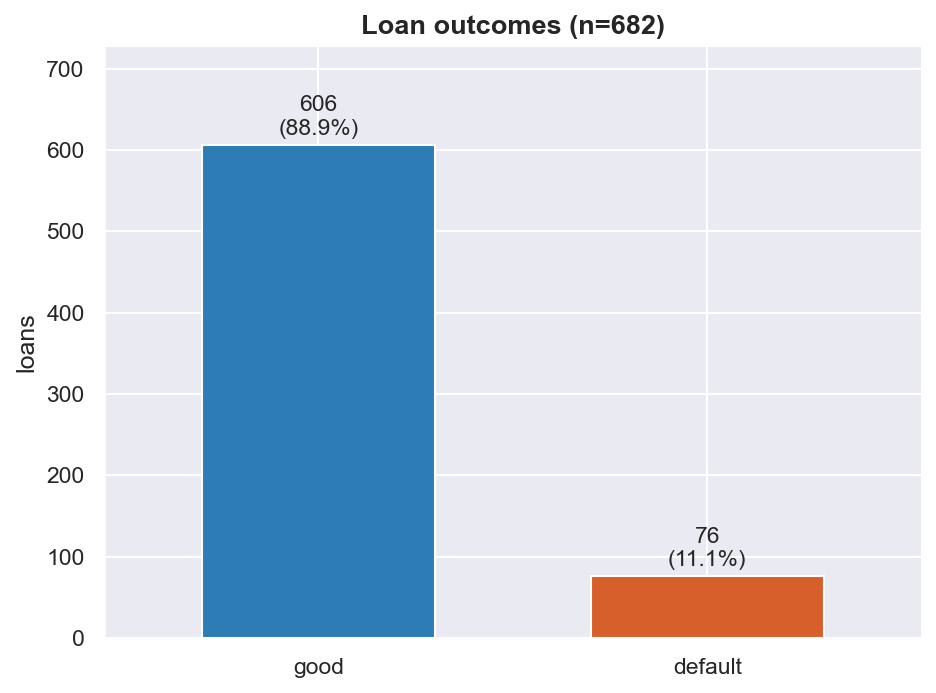
\includegraphics[width=0.62\textwidth]{target_dist.png}
    \caption{Distribution of the binary target: 606 good loans and 76 defaults (11.14\%).}
    \label{fig:target-dist}
\end{figure}

\section{Features Associated with Default}
\label{sec:target-correlations}

Figure~\ref{fig:corr-target} ranks the numeric features by their Pearson correlation with the default label. The strongest associations are negative and involve account balance: \texttt{min\_balance} at $-0.26$, \texttt{balance\_at\_loan} at $-0.20$, and \texttt{avg\_balance} at $-0.16$. Borrowers who defaulted tended to have lower balances before the loan, and the lowest point of their balance history was further below zero than for good borrowers.

On the loan side, \texttt{amount} correlates at $+0.17$ and \texttt{payments} at $+0.18$: larger loans and the higher monthly payments that come with them are associated with default. Age and gender are close to zero ($+0.01$ and $+0.02$), which is an early indication that the demographic variables carry little signal in this dataset.

\begin{figure}[H]
    \centering
    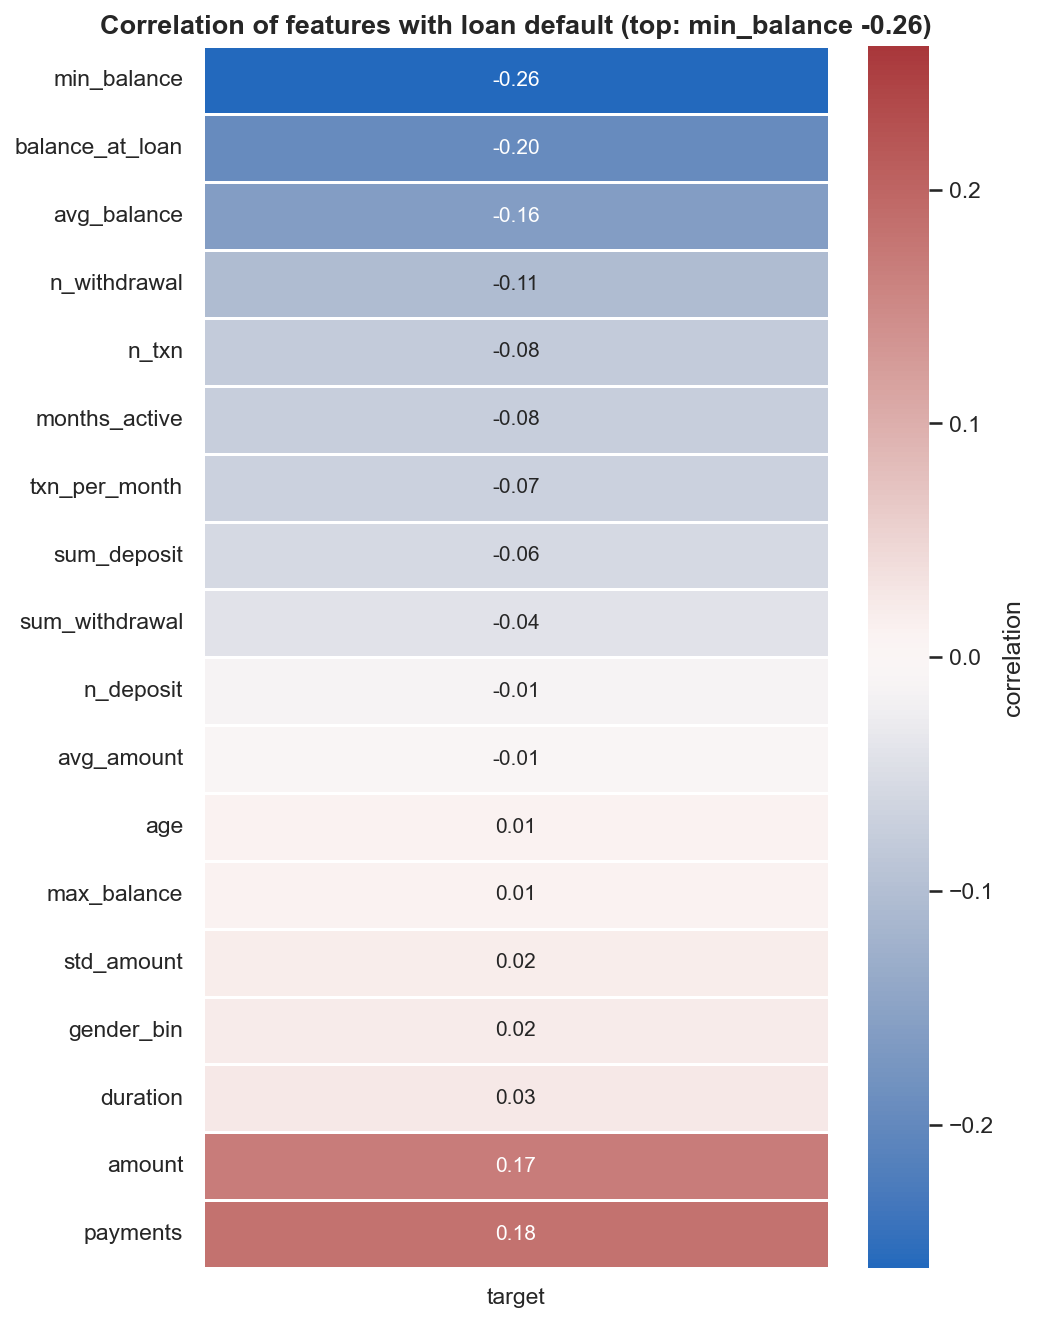
\includegraphics[width=0.62\textwidth]{corr_target.png}
    \caption{Correlation of each numeric feature with the default label. Balance features are negative; loan size and payment are positive.}
    \label{fig:corr-target}
\end{figure}

Correlation is a linear summary and can understate a relationship that is concentrated in a tail. The next two sections look at distributions rather than coefficients.

\section{Balance Separation}
\label{sec:balance-separation}

Figure~\ref{fig:behavior-box} compares the distributions of the main behavioural features for good and defaulted loans. The medians tell a consistent story. The balance at the loan date has a median of about 39,500 for good loans and 22,000 for defaults. Average balance is about 44,100 for good loans and 37,000 for defaults. The gap is not a handful of extreme accounts: the default distribution sits lower across its middle.

Transaction frequency barely separates the classes. Both groups transact at roughly 5.6 to 5.7 times per month. A busy account is not automatically a safe account. What matters more is the level of the balance and whether it was falling before the loan.

\begin{figure}[H]
    \centering
    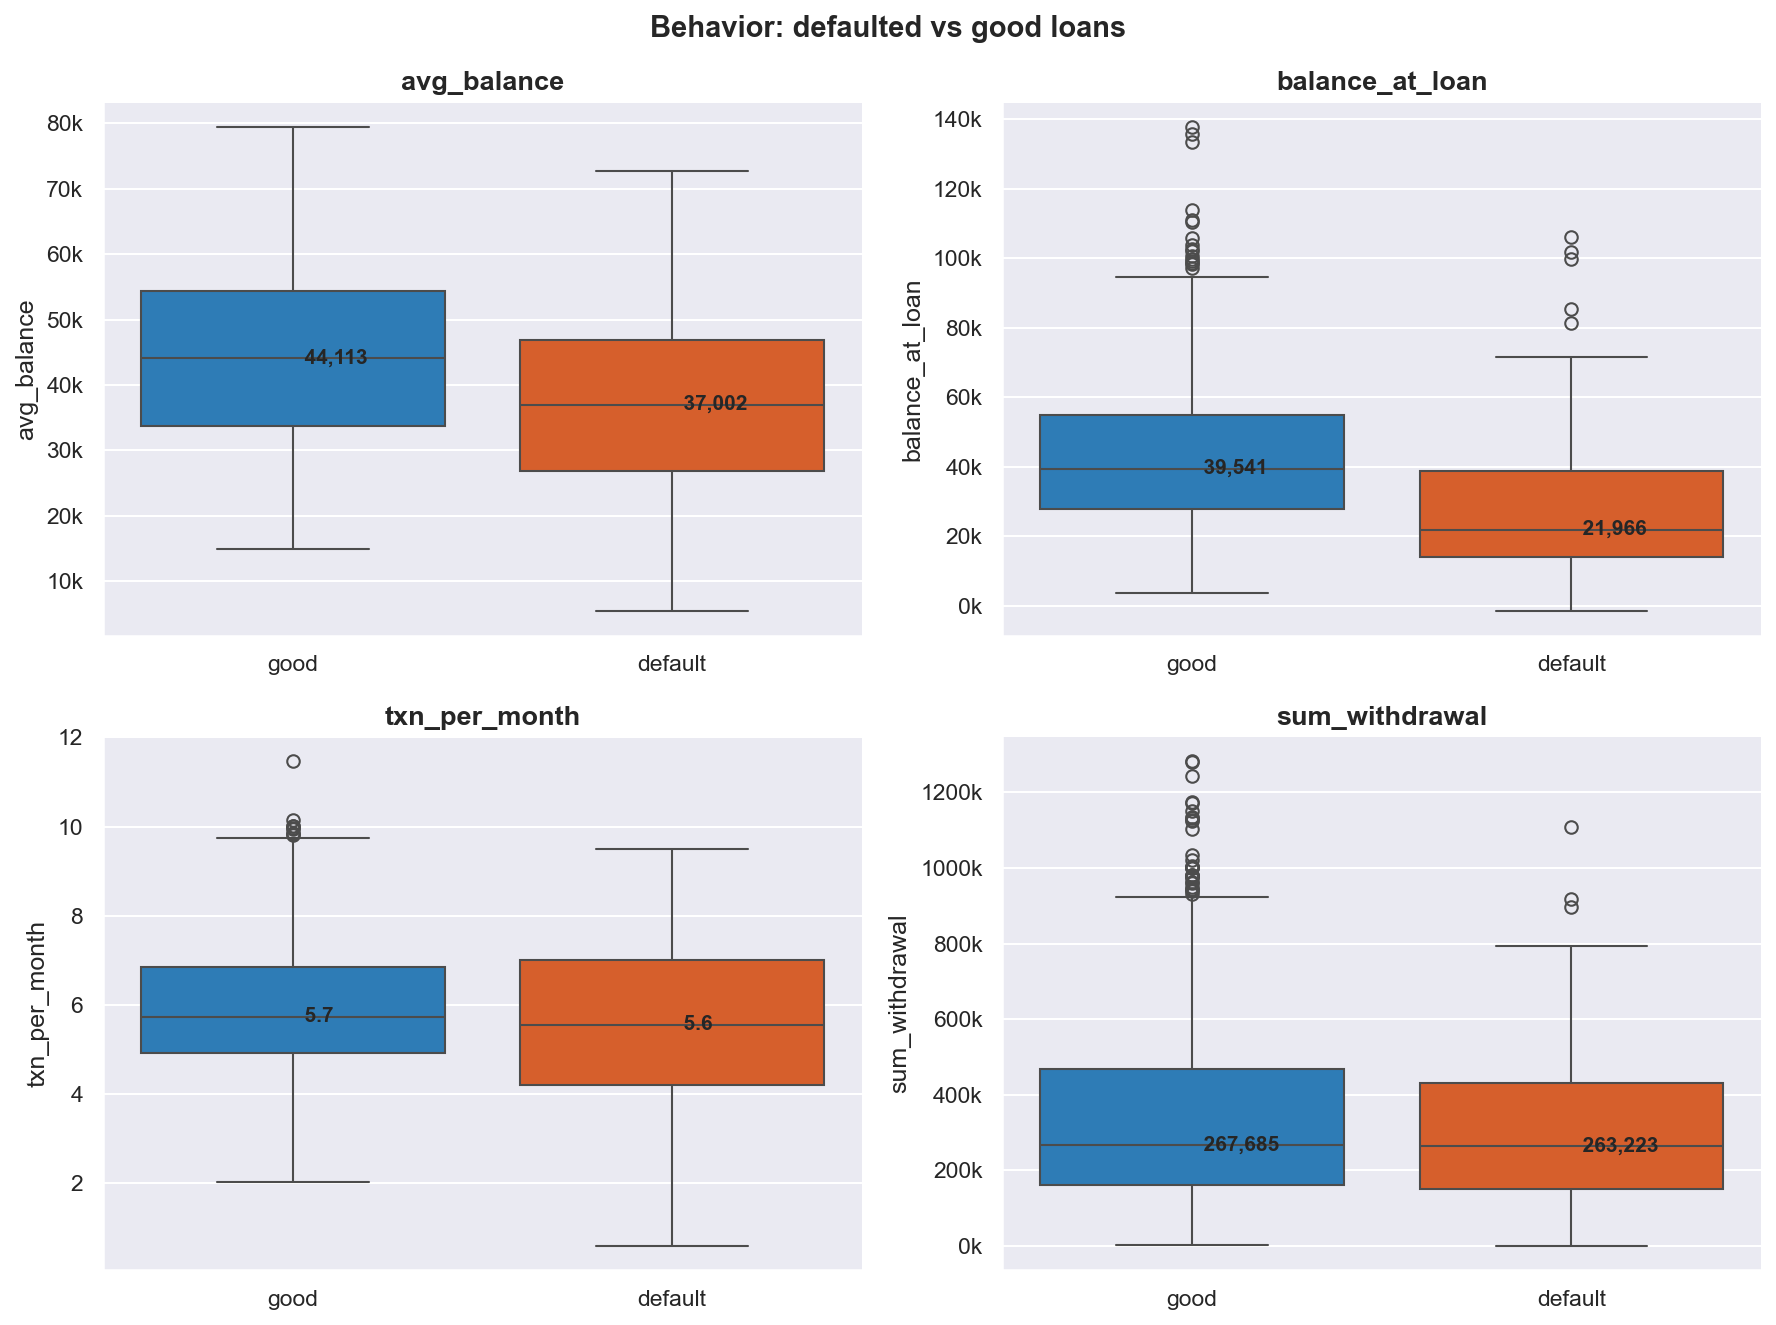
\includegraphics[width=0.9\textwidth]{behavior_box.png}
    \caption{Box plots of selected behavioural features by class. The balance distributions separate more clearly than transaction frequency.}
    \label{fig:behavior-box}
\end{figure}

\section{Age and Gender}
\label{sec:age-gender}

Figure~\ref{fig:age-hist} shows the age distribution split by outcome. Defaults appear across the full age range, with no concentration in a particular decade. The visual impression matches the near-zero correlation: age is not a useful discriminator on its own.

The gender split is similarly weak. Female borrowers default at 11.8\% and male borrowers at 10.5\%, a difference of 1.3 percentage points on a small minority class. With 76 defaults in total, that difference is well within sampling noise. Gender is kept as a feature for completeness, but the report does not build a business rule around it.

\begin{figure}[H]
    \centering
    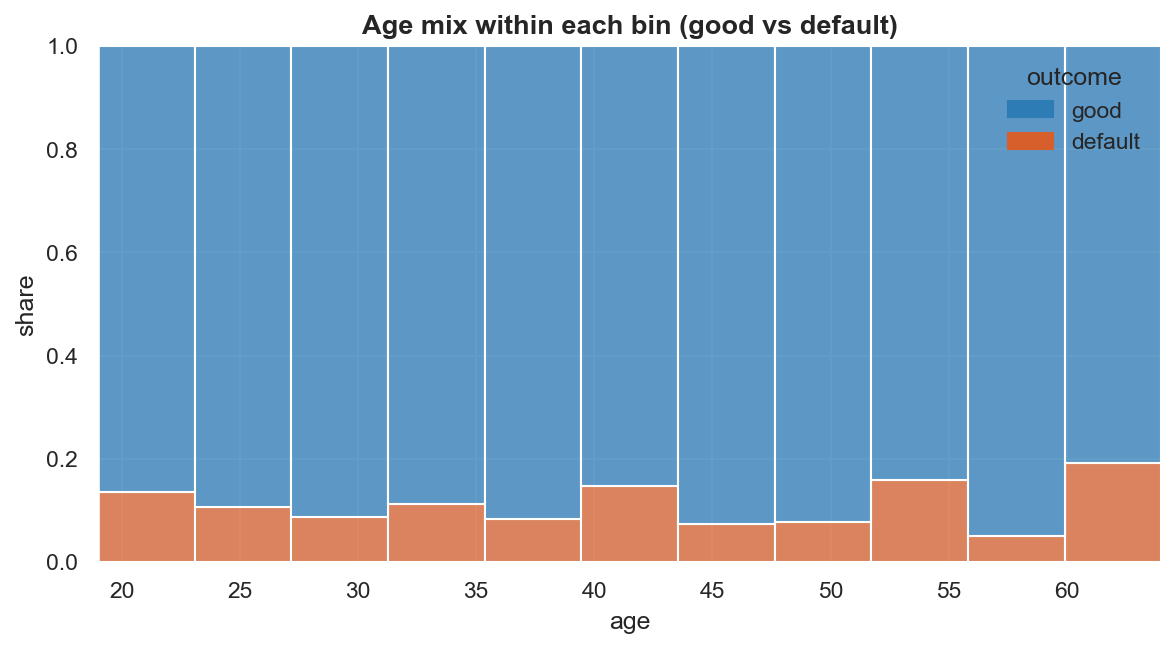
\includegraphics[width=0.75\textwidth]{age_hist.png}
    \caption{Age distribution by outcome. Defaults occur across all ages rather than in a single band.}
    \label{fig:age-hist}
\end{figure}

\section{Collinearity and Redundancy}
\label{sec:collinearity}

Figure~\ref{fig:corr-full} shows the full correlation matrix of the numeric features. Two clusters stand out. The first is the cash-flow pair: \texttt{sum\_deposit} and \texttt{sum\_withdrawal} correlate at 0.997, which is close to a duplicate. The second is the loan-burden pair: \texttt{amount} and \texttt{payments} move together, as they must under a fixed rate and duration.

The balance features form a softer cluster. \texttt{avg\_balance}, \texttt{min\_balance}, \texttt{max\_balance}, and \texttt{balance\_at\_loan} are related but not interchangeable; the minimum captures a different part of the distribution than the last observed value. This is why all four are retained, even though their importance scores will partly overlap.

\begin{figure}[H]
    \centering
    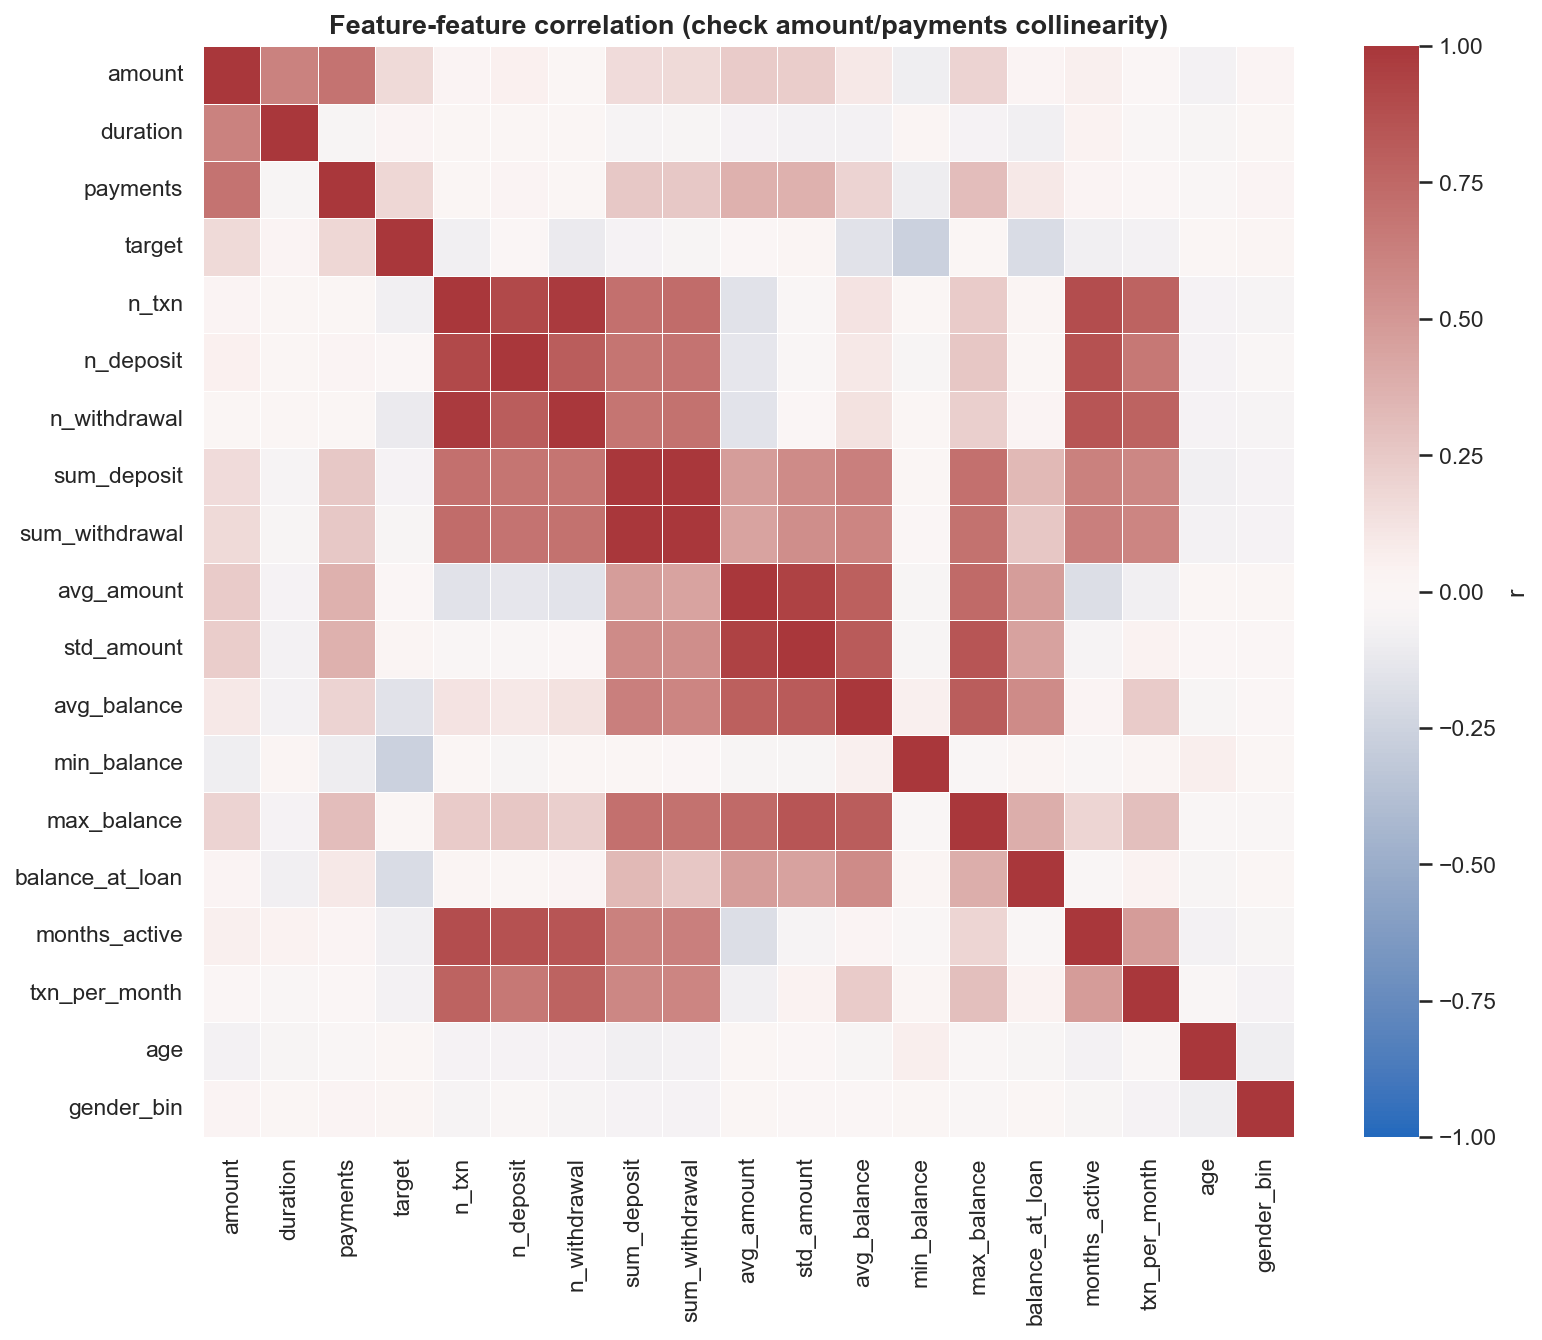
\includegraphics[width=0.85\textwidth]{corr_full.png}
    \caption{Correlation matrix of the numeric features. The cash-flow pair is nearly duplicated, and loan amount tracks monthly payment.}
    \label{fig:corr-full}
\end{figure}

The redundancy has a practical consequence for interpretation. When two features carry almost the same information, a tree can split on either one, and the reported importance can move between them across runs. The feature importance discussion in Chapter~\ref{ch:models} therefore groups related variables rather than treating each score as a separate causal effect.

\section{Loan Size Relative to Balance}
\label{sec:risk-quadrant}

The two strongest themes in the univariate analysis are balance level and loan size. Figure~\ref{fig:risk-quadrant} combines them. Loans are split at the median pre-loan balance of about 38,500 and the median loan amount of about 116,900. The four cells have very different default rates.

\begin{table}[H]
    \centering
    \caption{Default rate by pre-loan balance and loan amount, split at the respective medians.}
    \label{tab:risk-quadrant}
    \begin{tabular}{@{}llr@{}}
        \toprule
        \textbf{Balance} & \textbf{Loan amount} & \textbf{Default rate} \\
        \midrule
        High & Low & 4.9\% \\
        High & High & 6.7\% \\
        Low & Low & 10.1\% \\
        Low & High & 23.3\% \\
        \bottomrule
    \end{tabular}
\end{table}

The highest-risk cell is the borrower with a below-median balance asking for an above-median loan. Its default rate of 23.3\% is more than double the base rate and roughly five times the rate in the high-balance, low-amount cell. The pattern is intuitive: the loan is large relative to the buffer the account has shown. It also suggests a simple screening rule that does not require a model, which is useful as a sanity check on whatever the classifiers learn.

\begin{figure}[H]
    \centering
    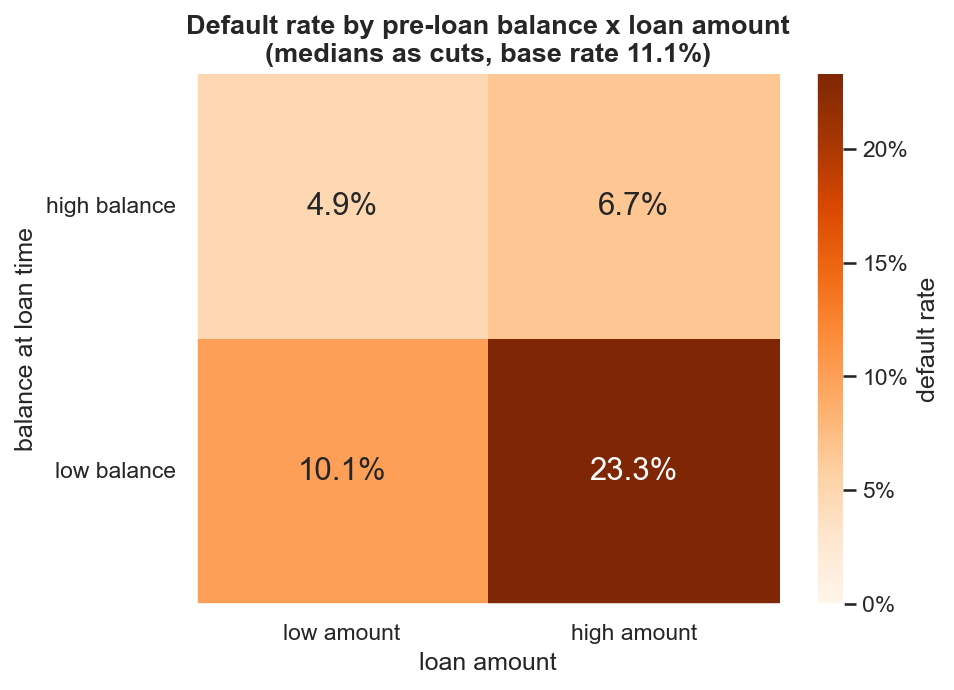
\includegraphics[width=0.62\textwidth]{risk_quadrant.png}
    \caption{Default rate by balance and loan amount. The low-balance, high-amount quadrant has the highest risk.}
    \label{fig:risk-quadrant}
\end{figure}

\section{Behavioural Segments}
\label{sec:segments}

A KMeans clustering with two groups was fitted on the behavioural and loan variables, with the target excluded. The silhouette score of 0.29 is modest, so the segments should be read as a coarse summary rather than as natural kinds. Figure~\ref{fig:segments-scatter} shows the separation in the balance and activity space, and Table~\ref{tab:segment-profiles} gives the profiles.

\begin{table}[H]
    \centering
    \caption{Profiles of the two behavioural segments. The target was not used to form the clusters.}
    \label{tab:segment-profiles}
    \begin{tabular}{@{}lrrrrr@{}}
        \toprule
        \textbf{Segment} & \textbf{Loans} & \textbf{Median txns} & \textbf{Mean balance} & \textbf{Txns/month} & \textbf{Default rate} \\
        \midrule
        0 & 421 & 54 & 37,200 & 5.2 & 12.4\% \\
        1 & 261 & 116 & 52,400 & 6.9 & 9.2\% \\
        \bottomrule
    \end{tabular}
\end{table}

Segment 0 is the larger, quieter group: fewer transactions, lower average balance, and a default rate of 12.4\%. Segment 1 is more active and holds a higher balance, with a default rate of 9.2\%. The direction is sensible, but the overlap is substantial. Activity alone does not separate the classes cleanly, which is consistent with the weak univariate correlation of \texttt{txn\_per\_month}. The segment label is useful for describing the portfolio, not for deciding a loan.

\begin{figure}[H]
    \centering
    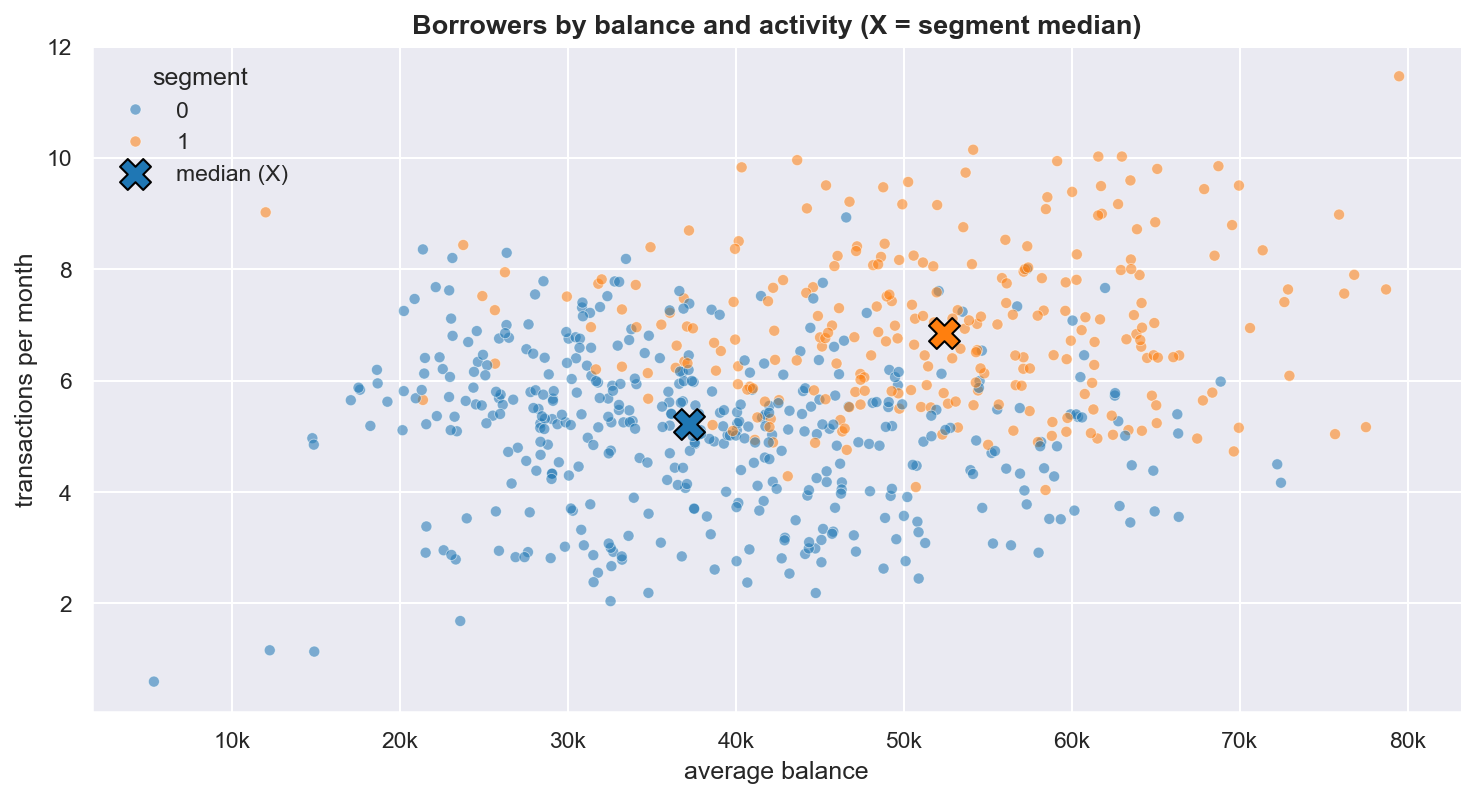
\includegraphics[width=0.9\textwidth]{segments_scatter.png}
    \caption{Loans in the two behavioural segments, plotted in the activity and balance space.}
    \label{fig:segments-scatter}
\end{figure}

\begin{figure}[H]
    \centering
    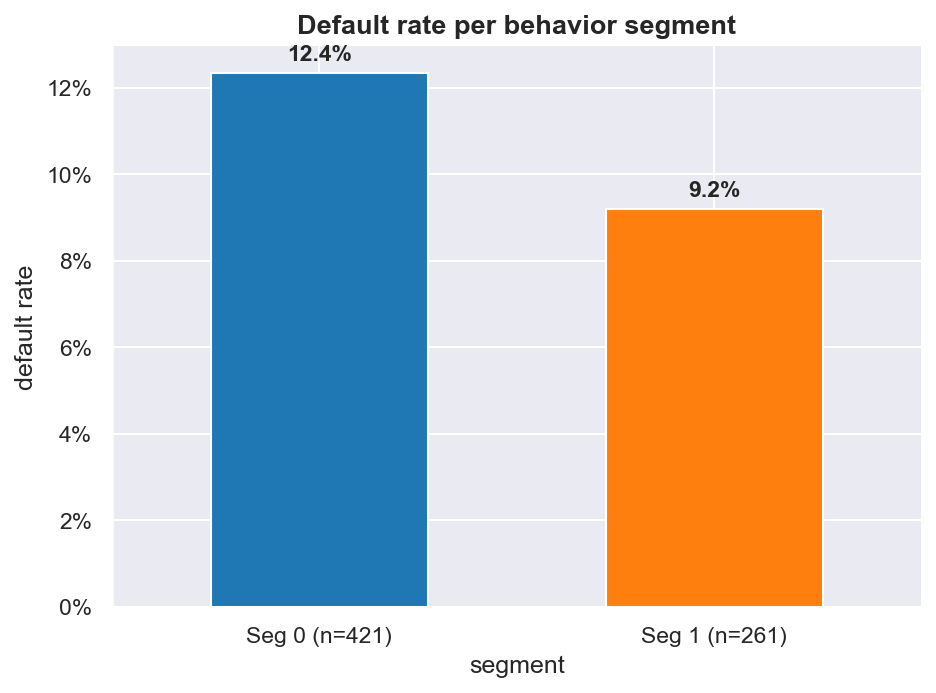
\includegraphics[width=0.62\textwidth]{segments_default.png}
    \caption{Default rate by segment. The quieter, lower-balance segment has the higher rate, but the difference is modest.}
    \label{fig:segments-default}
\end{figure}

\section{Summary of Findings}
\label{sec:eda-summary}

The exploratory work supports five conclusions that carry into the modelling chapter.

\begin{itemize}
    \item Balance history is the main behavioural axis. \texttt{min\_balance} and \texttt{balance\_at\_loan} have the strongest correlations with default, and their distributions separate visibly.
    \item Loan size matters in combination with balance. The low-balance, high-amount quadrant reaches a 23.3\% default rate, far above the 11.14\% base rate.
    \item Age and gender carry little signal. Their correlations are near zero and the age distribution shows no high-risk band.
    \item Activity volume is weak on its own. Transaction frequency is similar across classes, and the two clusters differ by only about three percentage points in default rate.
    \item Collinearity is present but manageable. The cash-flow pair is nearly duplicated, and the balance features overlap; interpretation should focus on groups of related variables.
\end{itemize}

These findings set expectations for the classifiers. A model should improve on the base rate mainly by using balance and loan burden, should not gain much from demographics, and should be judged on its ability to catch the small default class rather than on overall accuracy.

% Chapter 6
\chapter{Classification Models and Performance Evaluation}
\label{ch:models}

This chapter compares six classifiers under two imbalance strategies. It first describes the configurations and the training protocol, then reports the performance metrics, the held-out test results, the repeated cross-validation results, the ranking curves, the feature importance analysis, and the pattern matching results. The chapter closes with an interpretation of what the numbers do and do not support.

\section{Classifiers and Configurations}
\label{sec:classifiers}

Six classifiers were chosen to cover different inductive biases: a single tree, a probabilistic baseline, a bagged ensemble, a margin-based method, an instance-based method, and a boosted ensemble. Table~\ref{tab:classifiers} lists them and the reason each was included.

\begin{table}[H]
    \centering
    \caption{Classifiers evaluated in the project.}
    \label{tab:classifiers}
    \begin{tabularx}{\textwidth}{@{}lX@{}}
        \toprule
        \textbf{Classifier} & \textbf{Implementation and role} \\
        \midrule
        Decision Tree & \texttt{DecisionTreeClassifier}. A single axis-aligned tree. It is the most interpretable model in the set and provides a non-ensemble reference point. \\
        Naive Bayes & \texttt{GaussianNB}. A fast probabilistic baseline that assumes conditional independence of the features. \\
        Random Forest & \texttt{RandomForestClassifier}. A bagged ensemble of deep trees. It captures interactions and is robust to irrelevant features. \\
        Support Vector Machine & \texttt{SVC}, wrapped in \texttt{CalibratedClassifierCV}. A margin-based classifier with RBF and linear kernels. It requires scaled inputs. \\
        K-Nearest Neighbours & \texttt{KNeighborsClassifier}. An instance-based classifier that labels a loan by the majority of its nearest neighbours. It also requires scaled inputs. \\
        Gradient Boosting & \texttt{GradientBoostingClassifier}. A sequential ensemble that fits each tree to the residual of the previous ones. \\
        \bottomrule
    \end{tabularx}
\end{table}

Each classifier is evaluated under two imbalance settings. The baseline arm trains on the natural class distribution. The SMOTE arm applies Synthetic Minority Over-sampling Technique inside the pipeline, so the minority class is oversampled to parity within each training fold. The combination gives six models times two settings, or twelve configurations.

The SVM is wrapped in a calibrator because the probability estimates of \texttt{SVC} were deprecated in recent scikit-learn releases. The calibrator is fitted inside the pipeline and does not see the validation fold.

\section{Training Pipeline}
\label{sec:training-pipeline}

The pipeline for each configuration has four steps: optional scaling, optional SMOTE, the classifier, and prediction. Scaling is included for SVM and KNN and omitted for the tree models, which do not need it. The order matters: SMOTE is applied after scaling, so the synthetic points are generated in the same coordinate system as the real ones, and both steps are fitted only on the training portion of each split.

The protocol has three stages.

\begin{enumerate}
    \item \textbf{Single split.} All twelve configurations are trained on the 511-loan training partition with default hyperparameters and scored on the 171-loan test partition.
    \item \textbf{Hyperparameter search.} For each configuration, \texttt{RandomizedSearchCV} samples up to 30 parameter combinations and scores them with F1 on an inner five-fold stratified cross-validation of the training partition. The search never touches the test partition. Naive Bayes has 9 candidates and KNN has 24 because their grids are small.
    \item \textbf{Repeated cross-validation.} The default and tuned versions of all twelve configurations are evaluated with five-fold stratified cross-validation repeated ten times. This produces 50 F1 estimates per configuration and is the table used to select the final model.
\end{enumerate}

The selection metric is mean F1 from the repeated cross-validation. Average precision and ROC-AUC are reported alongside it, but they are not used to re-rank the models after the fact. Fixing the criterion before seeing the results avoids choosing whichever metric happens to favour a preferred model.

\section{Hyperparameter Tuning}
\label{sec:tuning}

Table~\ref{tab:tuning-results} lists the best configuration found for each model and imbalance setting, the number of candidates evaluated, the inner cross-validation F1, and the selected parameters. The search is deliberately modest: 30 candidates per configuration is enough to show whether tuning helps, without turning a 511-row training set into a long optimisation exercise.

\begin{table}[H]
    \centering
    \caption{Hyperparameter search results, ranked by inner cross-validation F1.}
    \label{tab:tuning-results}
    \small
    \begin{tabularx}{\textwidth}{@{}l l r c X@{}}
        \toprule
        \textbf{Model} & \textbf{Arm} & \textbf{Cand.} & \textbf{Inner F1} & \textbf{Best parameters} \\
        \midrule
        Gradient Boosting & Baseline & 30 & 0.582 & \texttt{subsample=0.7; n\_estimators=300; max\_depth=1; learning\_rate=0.05} \\
        Random Forest & SMOTE & 30 & 0.576 & \texttt{n\_estimators=200; min\_samples\_leaf=5; max\_features=sqrt; max\_depth=20} \\
        Gradient Boosting & SMOTE & 30 & 0.538 & \texttt{subsample=0.7; n\_estimators=300; max\_depth=2; learning\_rate=0.05} \\
        SVM & SMOTE & 30 & 0.530 & \texttt{kernel=linear; gamma=0.01; C=100} \\
        Random Forest & Baseline & 30 & 0.519 & \texttt{n\_estimators=200; min\_samples\_leaf=1; max\_features=log2; max\_depth=8} \\
        Decision Tree & SMOTE & 30 & 0.510 & \texttt{min\_samples\_leaf=2; max\_depth=12; criterion=gini; class\_weight=None} \\
        SVM & Baseline & 30 & 0.503 & \texttt{kernel=rbf; gamma=0.01; C=0.1} \\
        Decision Tree & Baseline & 30 & 0.492 & \texttt{min\_samples\_leaf=5; max\_depth=3; criterion=gini; class\_weight=None} \\
        KNN & SMOTE & 24 & 0.385 & \texttt{weights=distance; p=2; n\_neighbors=21} \\
        Naive Bayes & Baseline & 9 & 0.371 & \texttt{var\_smoothing=1e-11} \\
        Naive Bayes & SMOTE & 9 & 0.321 & \texttt{var\_smoothing=1e-11} \\
        KNN & Baseline & 24 & 0.229 & \texttt{weights=uniform; p=2; n\_neighbors=3} \\
        \bottomrule
    \end{tabularx}
\end{table}

The strongest inner-CV result belongs to Gradient Boosting without resampling: 0.582 with a shallow model of 300 stumps, a learning rate of 0.05, and 70\% subsampling. The selected depth of one means each boosting round adds a single split, which keeps the model close to an additive model and limits overfitting on 511 rows.

The tuning curves in Figure~\ref{fig:tuning-curves} show F1 against the key hyperparameter for the two strongest families. The curves are flat over much of the range and then fall sharply. That shape is a warning against reading too much into a small difference between neighbouring settings: the surface is noisy, and the inner CV has only 57 defaults to work with.

\begin{figure}[H]
    \centering
    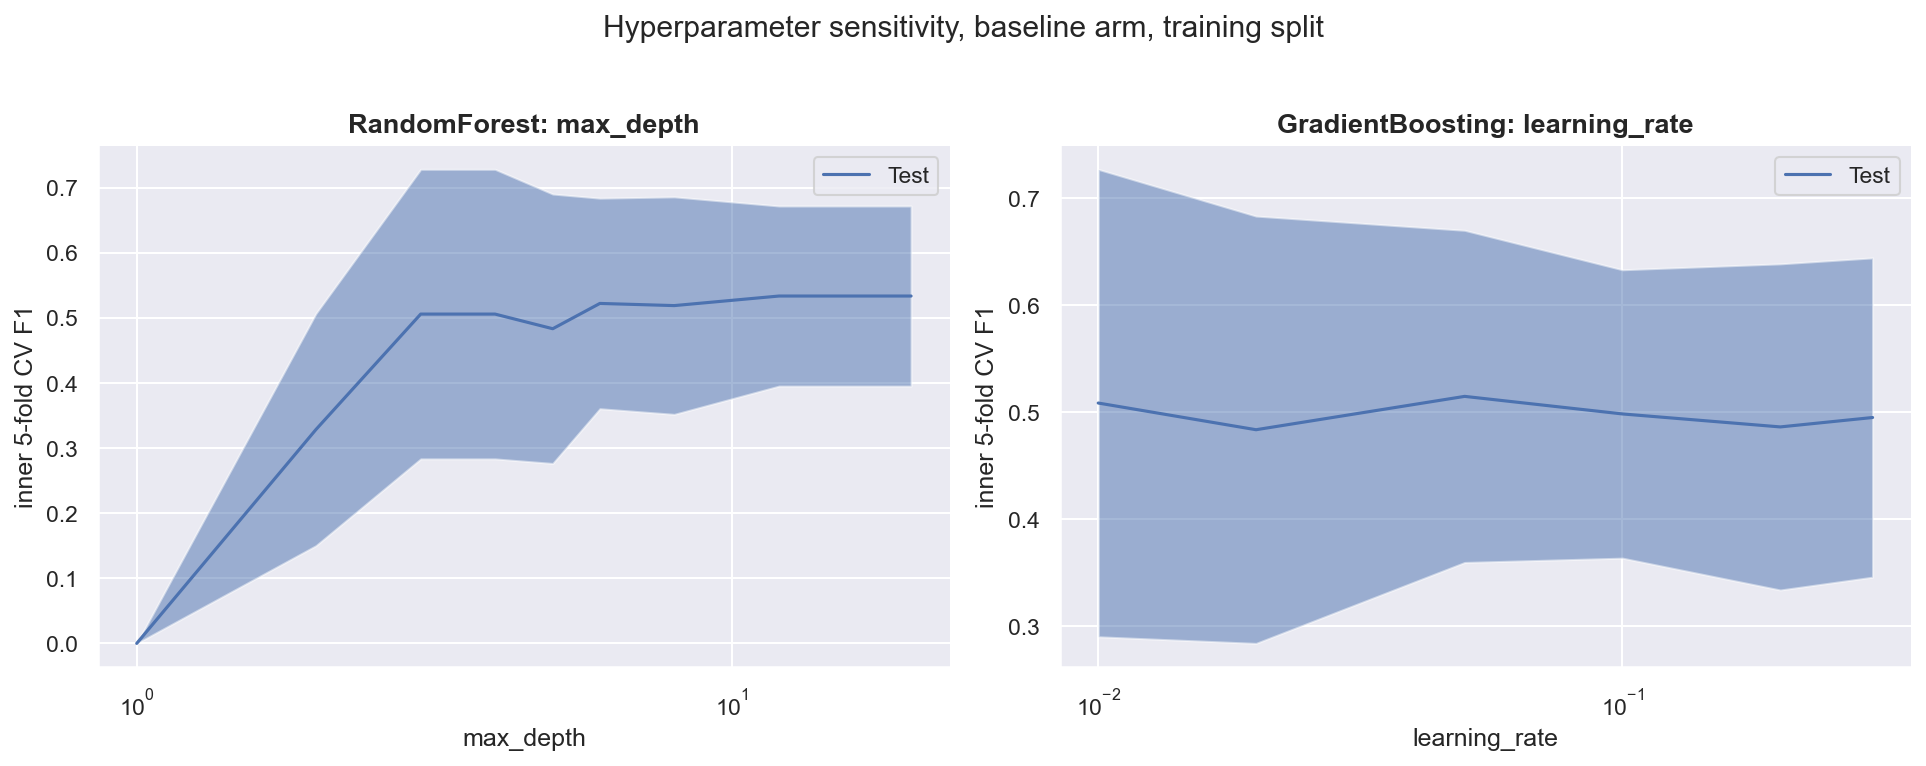
\includegraphics[width=0.95\textwidth]{tuning_curves.png}
    \caption{Hyperparameter sensitivity for the baseline arm on the training split. F1 is flat over a broad region and falls at the extremes.}
    \label{fig:tuning-curves}
\end{figure}

\section{Performance Metrics and Held-Out Test Results}
\label{sec:test-results}

Table~\ref{tab:test-results} reports the single-split results for all twelve configurations with default hyperparameters. The test partition has 171 loans, 19 of which defaulted. A single default therefore moves recall by about 5.3 percentage points, which is the scale against which differences should be read.

\begin{table}[H]
    \centering
    \caption{Held-out test performance with default hyperparameters (171 loans, 19 defaults).}
    \label{tab:test-results}
    \small
    \begin{tabular}{@{}l l r r r r r r@{}}
        \toprule
        \textbf{Model} & \textbf{Arm} & \textbf{Acc.} & \textbf{Prec.} & \textbf{Rec.} & \textbf{F1} & \textbf{AP} & \textbf{AUC} \\
        \midrule
        Random Forest & Baseline & 0.924 & 0.875 & 0.368 & 0.519 & 0.582 & 0.856 \\
        Decision Tree & Baseline & 0.895 & 0.529 & 0.474 & 0.500 & 0.309 & 0.711 \\
        Gradient Boosting & Baseline & 0.912 & 0.700 & 0.368 & 0.483 & 0.583 & 0.816 \\
        SVM & Baseline & 0.918 & 0.857 & 0.316 & 0.462 & 0.551 & 0.771 \\
        Naive Bayes & Baseline & 0.807 & 0.150 & 0.158 & 0.154 & 0.171 & 0.634 \\
        KNN & Baseline & 0.895 & 1.000 & 0.053 & 0.100 & 0.220 & 0.668 \\
        Gradient Boosting & SMOTE & 0.889 & 0.500 & 0.421 & 0.457 & 0.495 & 0.741 \\
        Decision Tree & SMOTE & 0.883 & 0.471 & 0.421 & 0.444 & 0.262 & 0.681 \\
        Random Forest & SMOTE & 0.895 & 0.538 & 0.368 & 0.438 & 0.532 & 0.826 \\
        SVM & SMOTE & 0.854 & 0.375 & 0.474 & 0.419 & 0.385 & 0.726 \\
        KNN & SMOTE & 0.743 & 0.195 & 0.421 & 0.267 & 0.156 & 0.645 \\
        Naive Bayes & SMOTE & 0.591 & 0.108 & 0.368 & 0.167 & 0.155 & 0.563 \\
        \bottomrule
    \end{tabular}
\end{table}

The Random Forest has the highest accuracy (0.924) and precision (0.875), but it catches only 7 of the 19 defaults (recall 0.368). The Decision Tree catches 9 of 19 (recall 0.474) at a lower precision, which gives it the second-best F1. The Gradient Boosting sits between them with an F1 of 0.483 and the highest average precision of the baseline arm (0.583).

The KNN baseline illustrates why precision alone is misleading. It reports a precision of 1.000 because it predicts a single default and gets it right, but its recall is 0.053. A credit team could not use a model that reviews one case and misses eighteen.

SMOTE raises recall for most models but lowers precision by more. The Gradient Boosting arm moves from a recall of 0.368 to 0.421 while precision falls from 0.700 to 0.500. The net F1 is lower. The Naive Bayes SMOTE model is the clearest failure: accuracy falls to 0.591 and precision to 0.108, so the resampling has produced many false alarms without a useful gain in coverage.

Figure~\ref{fig:confusion-matrices} shows the confusion matrices for the twelve configurations. The top row, which contains the baseline models, is dominated by false negatives for the high-precision models. The SMOTE row shifts errors toward false positives. Neither error type is free: a false negative is a missed risky loan, while a false positive is a good customer sent to manual review.

\begin{figure}[H]
    \centering
    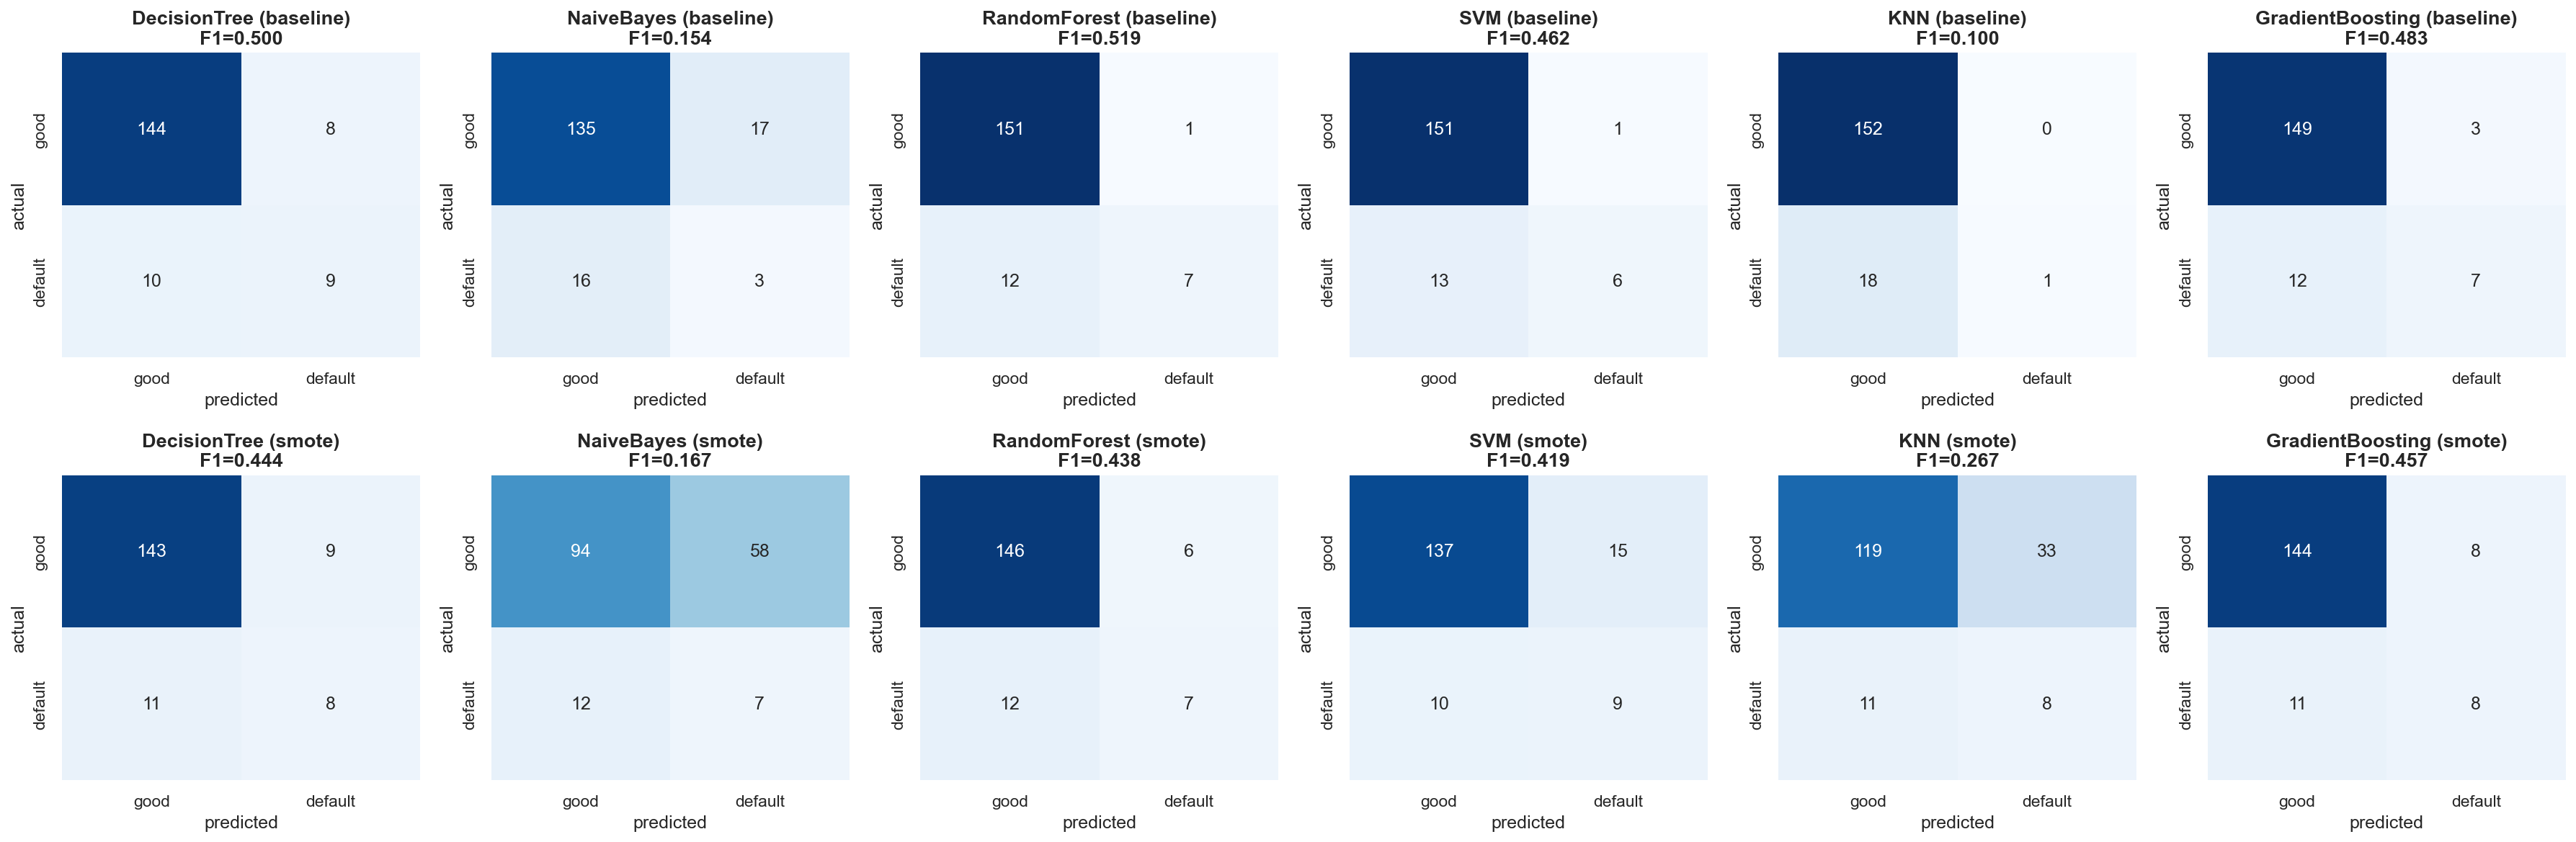
\includegraphics[width=0.95\textwidth]{confusion_matrices.png}
    \caption{Confusion matrices on the held-out test set with default hyperparameters. The two rows show the baseline and SMOTE arms.}
    \label{fig:confusion-matrices}
\end{figure}

\section{Validation Test: Repeated Cross-Validation}
\label{sec:cv-results}

A single test set of 171 loans cannot reliably separate models whose F1 differs by two or three points. Table~\ref{tab:cv-results} therefore reports the mean and standard deviation of F1 over 50 estimates from five-fold cross-validation repeated ten times. The table is ranked by tuned F1, and it includes the default F1 for the same configuration so the effect of tuning is visible.

\begin{table}[H]
    \centering
    \caption{Repeated stratified five-fold cross-validation, ten repeats (50 estimates), ranked by tuned F1. The last two columns describe the tuned configuration.}
    \label{tab:cv-results}
    \small
    \begin{tabular}{@{}l l r r r r@{}}
        \toprule
        \textbf{Model} & \textbf{Arm} & \textbf{F1 default} & \textbf{F1 tuned} & \textbf{AP tuned} & \textbf{AUC tuned} \\
        \midrule
        Gradient Boosting & Baseline & 0.557 & 0.571 $\pm$ 0.120 & 0.654 & 0.864 \\
        Decision Tree & Baseline & 0.491 & 0.557 $\pm$ 0.126 & 0.507 & 0.748 \\
        Random Forest & Baseline & 0.557 & 0.556 $\pm$ 0.112 & 0.661 & 0.877 \\
        Random Forest & SMOTE & 0.537 & 0.542 $\pm$ 0.103 & 0.638 & 0.872 \\
        Gradient Boosting & SMOTE & 0.542 & 0.536 $\pm$ 0.101 & 0.641 & 0.851 \\
        SVM & Baseline & 0.421 & 0.498 $\pm$ 0.128 & 0.603 & 0.842 \\
        Decision Tree & SMOTE & 0.452 & 0.464 $\pm$ 0.104 & 0.307 & 0.741 \\
        SVM & SMOTE & 0.436 & 0.463 $\pm$ 0.084 & 0.608 & 0.848 \\
        KNN & SMOTE & 0.336 & 0.367 $\pm$ 0.065 & 0.367 & 0.768 \\
        Naive Bayes & Baseline & 0.325 & 0.325 $\pm$ 0.132 & 0.356 & 0.769 \\
        Naive Bayes & SMOTE & 0.318 & 0.318 $\pm$ 0.055 & 0.338 & 0.729 \\
        KNN & Baseline & 0.198 & 0.223 $\pm$ 0.129 & 0.249 & 0.628 \\
        \bottomrule
    \end{tabular}
\end{table}

Gradient Boosting with the baseline arm has the highest mean tuned F1 at 0.571. Random Forest is second at 0.556 and has the best average precision (0.661) and ROC-AUC (0.877). The F1 gap between them is 0.015, while the fold-to-fold standard deviation is about 0.11. The two models are effectively tied on F1, and the Random Forest ranks positives better. The selection rule nevertheless points to Gradient Boosting because F1 was fixed as the criterion before the comparison. The report keeps Random Forest as a credible alternative rather than pretending the choice is unambiguous.

The Decision Tree is the surprise of the table. Tuning raises its F1 from 0.491 to 0.557, a gain of 0.066, and places it third. Its average precision is only 0.507, however. The tree has learned a decision boundary that captures more defaults at the cost of a less reliable ranking. This is the clearest example of why F1 and AP should be read together: they answer different questions.

The tuning gains are uneven. The SVM improves by 0.077 and the Decision Tree by 0.066, while the Random Forest does not improve at all ($-0.001$) and Naive Bayes is unchanged. The models with strong default settings had less room to gain, and the search may simply have confirmed that their defaults were already appropriate for this sample size.

SMOTE helps only KNN at the tuned comparison (0.223 to 0.367). For the other five models, the tuned baseline arm is at least as good as the tuned SMOTE arm. The result is consistent with the test table and with the small absolute number of defaults: synthetic minority points can smooth a boundary that is already hard to estimate, and the extra recall often arrives with a larger loss in precision. The project therefore does not recommend SMOTE as a default for this dataset.

Figure~\ref{fig:cv-selection} shows the tuning gain for each configuration, with the selected model marked. The visual makes the two large gains (SVM and Decision Tree) and the flat response of the already-strong models easy to see.

\begin{figure}[H]
    \centering
    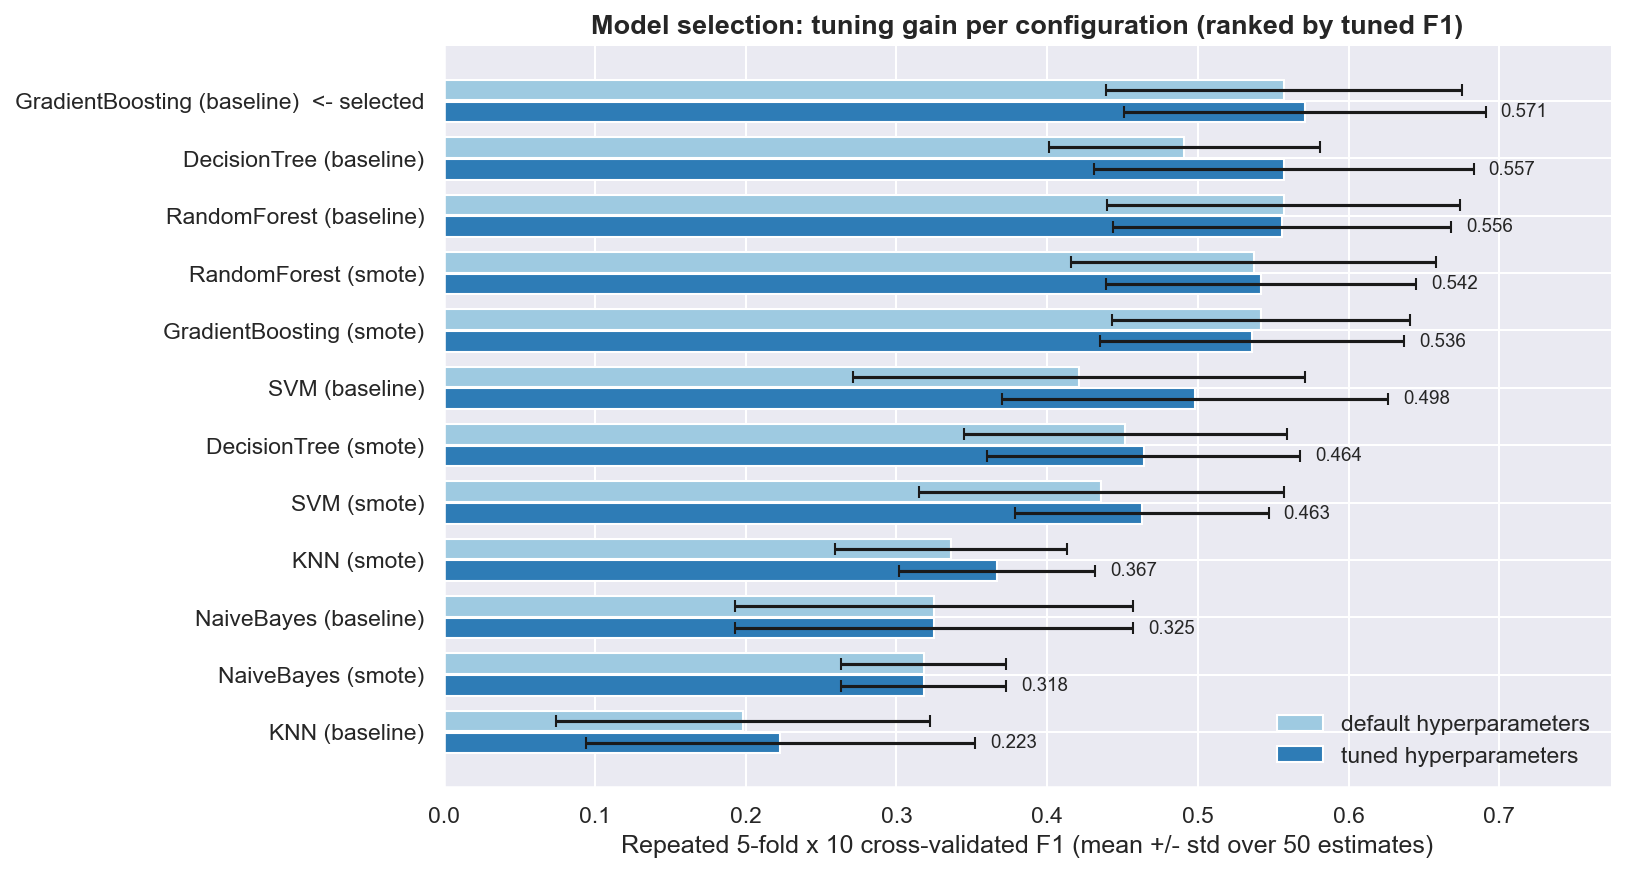
\includegraphics[width=0.9\textwidth]{cv_selection.png}
    \caption{Tuning gain per configuration under repeated cross-validation. The selected Gradient Boosting baseline is marked.}
    \label{fig:cv-selection}
\end{figure}

\section{Ranking Curves}
\label{sec:ranking-curves}

Figures~\ref{fig:roc-curves} and~\ref{fig:pr-curves} show the ROC and precision-recall curves for the default configurations. The ROC curves of Random Forest, Gradient Boosting, and SVM sit well above the diagonal, with AUC values in the 0.77 to 0.86 range on the test set. The precision-recall curves are more sobering. At an 11.14\% prevalence, the no-skill average precision is 0.111, and the best default model reaches about 0.58. That is a real improvement, but it is far from a clean separation.

\begin{figure}[H]
    \centering
    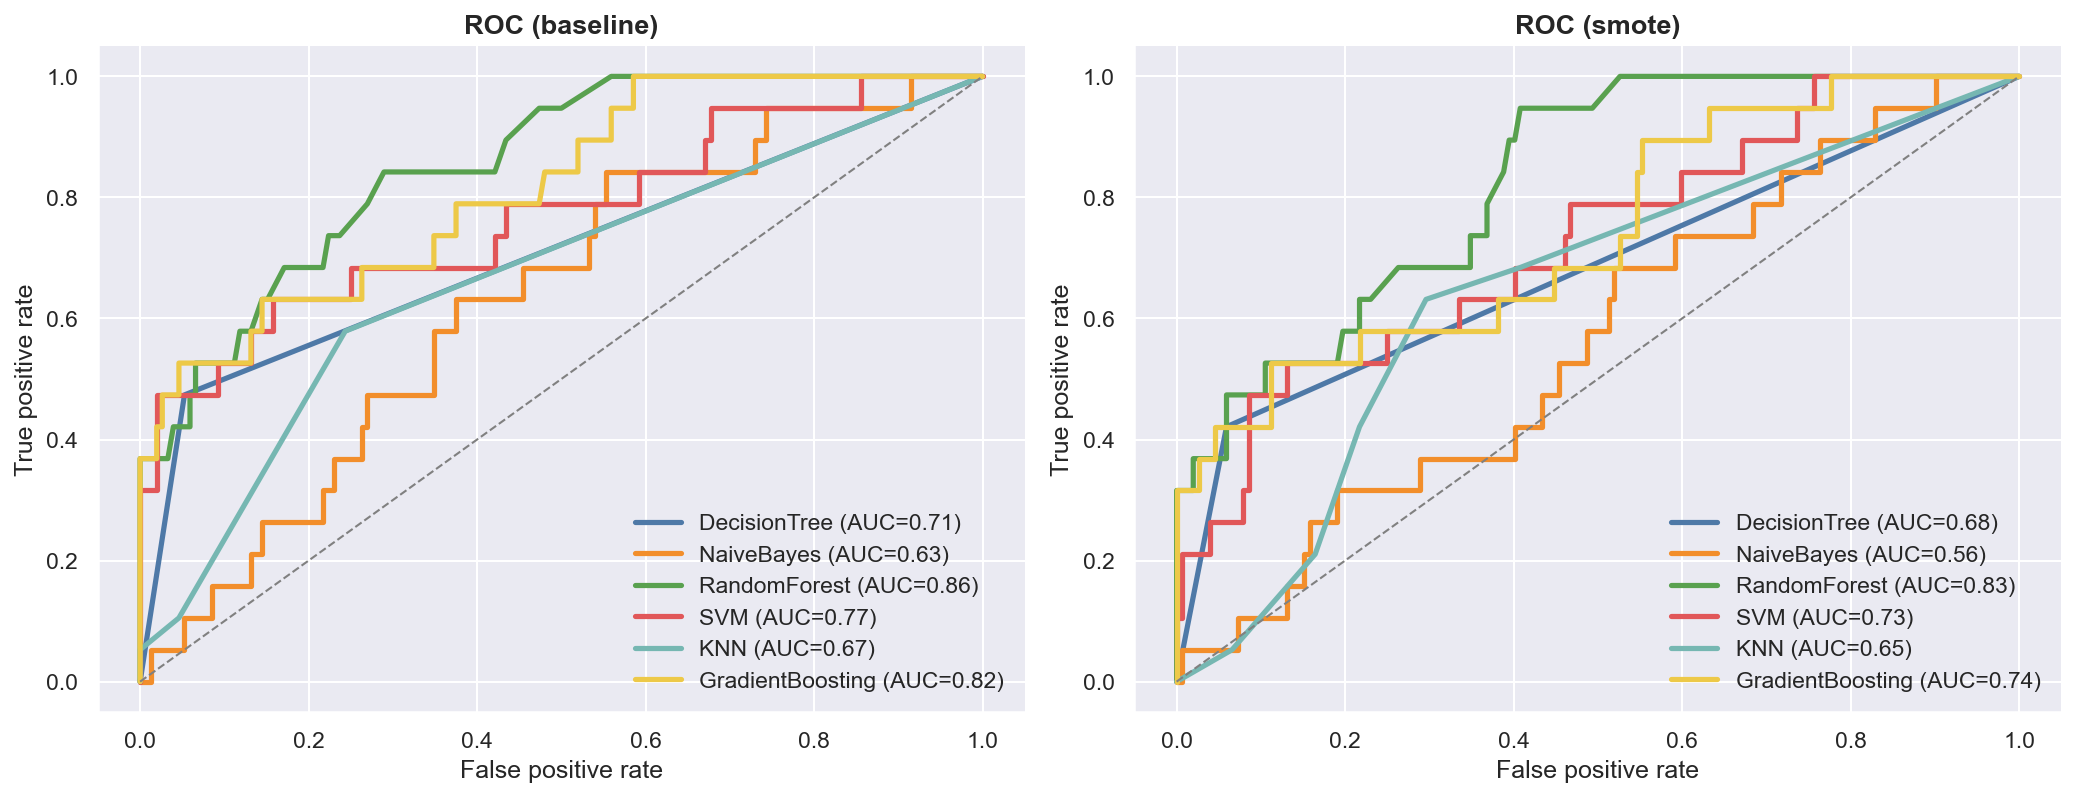
\includegraphics[width=0.95\textwidth]{roc_curves.png}
    \caption{ROC curves by imbalance arm on the held-out test set, default hyperparameters.}
    \label{fig:roc-curves}
\end{figure}

\begin{figure}[H]
    \centering
    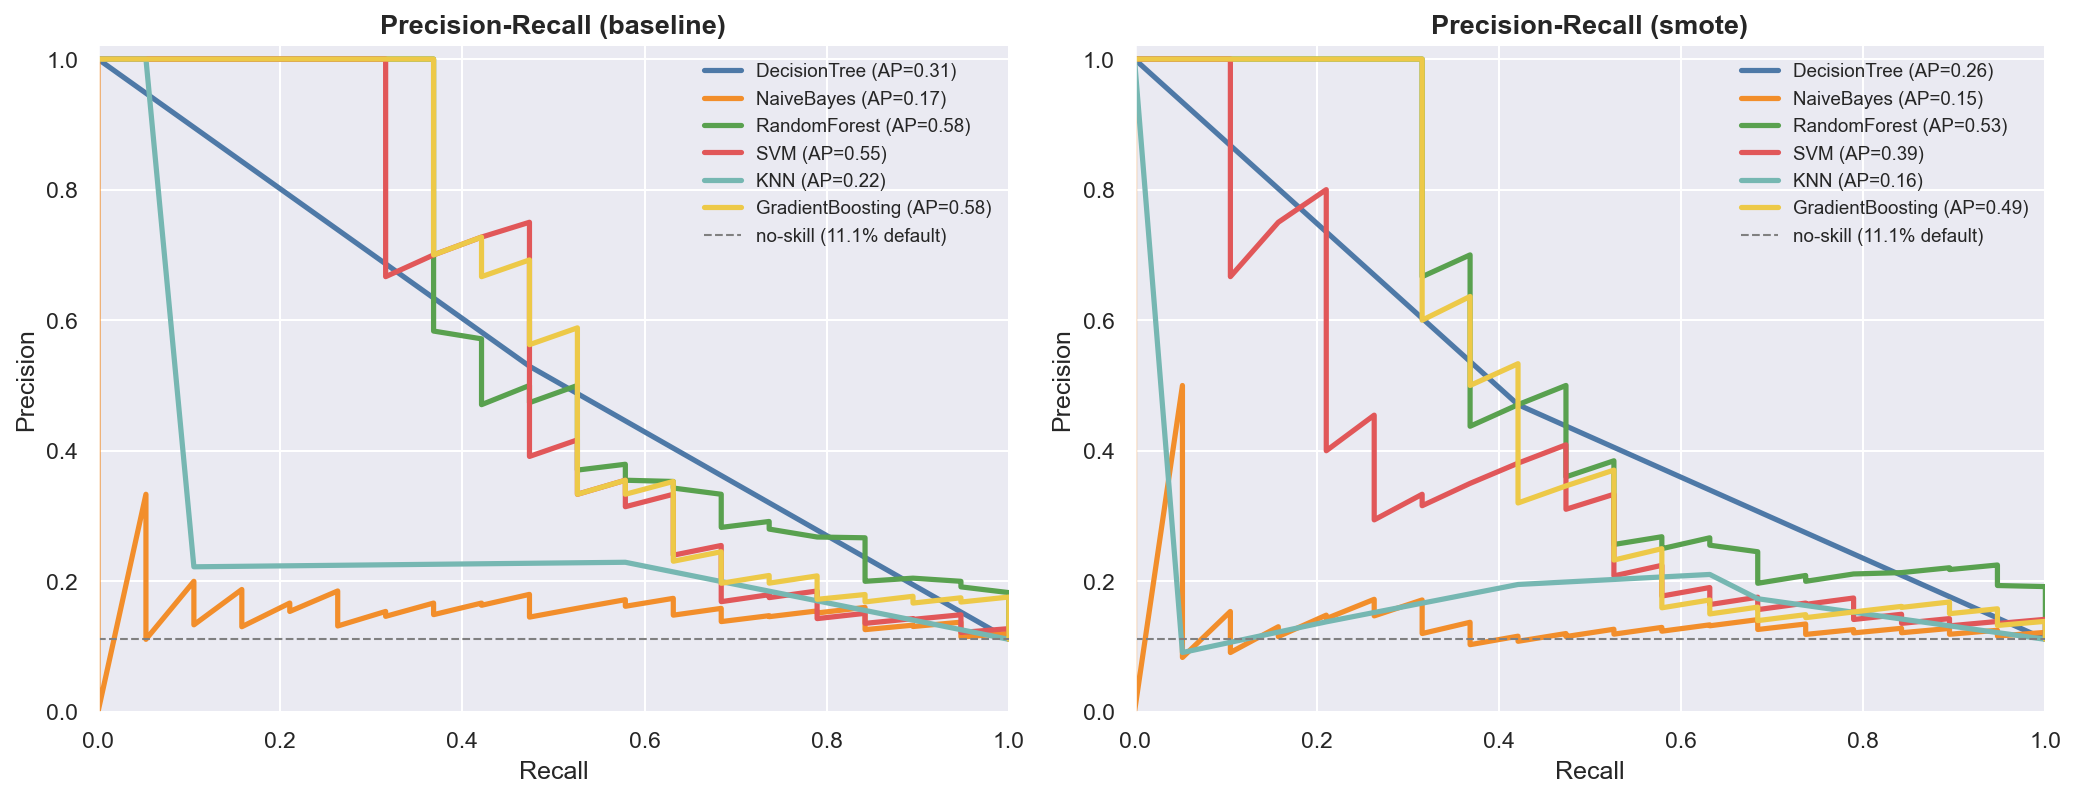
\includegraphics[width=0.95\textwidth]{pr_curves.png}
    \caption{Precision-recall curves with average precision on the held-out test set, default hyperparameters. The dashed baseline is the 11.14\% default rate.}
    \label{fig:pr-curves}
\end{figure}

The ROC view can flatter a model on imbalanced data because a large number of true negatives keeps the false-positive rate low even when many defaults are missed. The precision-recall view makes the cost visible: to reach a recall of 0.5, a model must accept a precision well below its peak. The operating threshold is therefore a business decision, not a property of the classifier.

\section{Feature Importance}
\label{sec:feature-importance}

Figure~\ref{fig:rf-importance} shows impurity-based importance from the tuned Random Forest. The Random Forest is used for this view because tree ensembles expose a direct importance score and the tuned forest was one of the two strongest models. The scores are not causal effects; they describe how much a feature contributed to reducing impurity across the forest.

\begin{figure}[H]
    \centering
    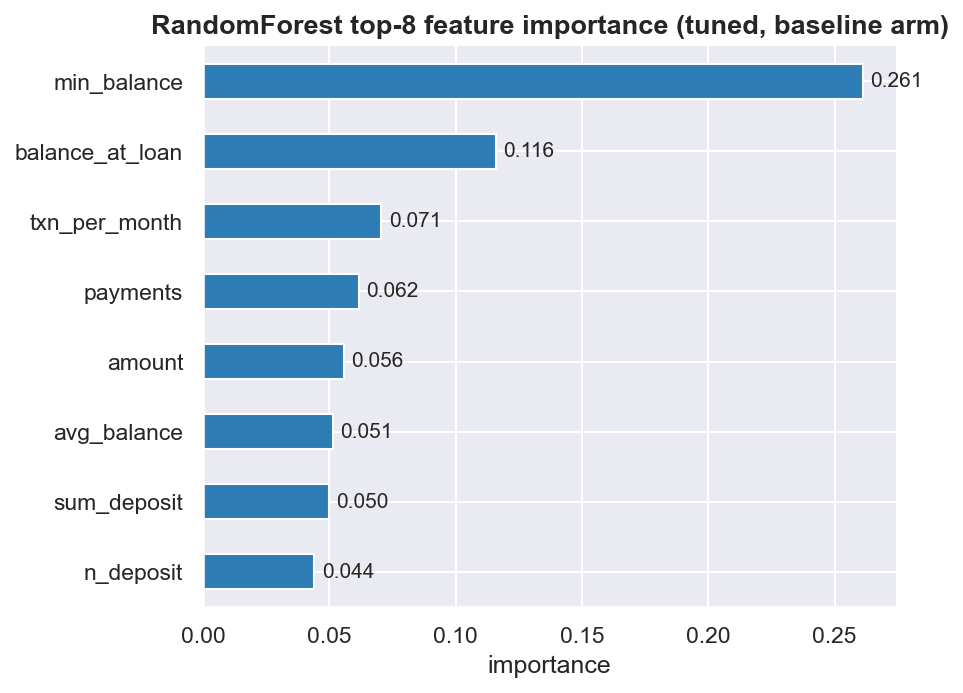
\includegraphics[width=0.62\textwidth]{rf_importance.png}
    \caption{Feature importance from the tuned Random Forest. Balance features dominate; demographic features contribute little.}
    \label{fig:rf-importance}
\end{figure}

\texttt{min\_balance} is the single most important feature at 0.261, followed by \texttt{balance\_at\_loan} at 0.116. The two balance features together account for more than a third of the total importance. Transaction frequency (0.071), monthly payment (0.062), loan amount (0.056), and average balance (0.051) form a second tier. Age (0.025) and gender (0.005) are near the bottom.

Two cautions apply. First, impurity importance is biased toward features with many distinct values, and all the money and count features are continuous. Second, correlated features share credit: when \texttt{sum\_deposit} and \texttt{sum\_withdrawal} carry almost the same information, the forest may split on either one, and their individual scores can change between runs. The grouped conclusion is safer than any single rank: balance history and loan burden carry the signal, while demographics do not.

\section{Pattern Matching with Apriori and FP-Growth}
\label{sec:pattern-mining}

The pattern mining step looks for simple co-occurrences between pre-loan behaviours and default. It uses Apriori and FP-Growth on one basket per account, built from the first loan on the account and transactions dated before that loan. An item records whether the account ever showed a behaviour in that window. The minimum support is 0.03, the maximum itemset length is three, the minimum confidence is 0.10, and rules are kept only if the lift is above 1.0 and the consequent is default. Redundant rules are pruned when a more general rule is at least as strong.

Both algorithms return the same 41 itemsets and the same two default-oriented rules, which is a useful consistency check. Table~\ref{tab:pattern-rules} reports the rules.

\begin{table}[H]
    \centering
    \caption{Default-oriented association rules after redundancy pruning. Support is the share of the 682 accounts; coverage is the share of the 76 defaults.}
    \label{tab:pattern-rules}
    \begin{tabular}{@{}l r r r r@{}}
        \toprule
        \textbf{Antecedent} & \textbf{Antecedent support} & \textbf{Confidence} & \textbf{Lift} & \textbf{Default coverage} \\
        \midrule
        \texttt{negative\_balance} & 3.96\% (27/682) & 100.0\% & 8.97 & 35.5\% (27/76) \\
        \texttt{type\_VYBER} & 54.11\% (369/682) & 13.0\% & 1.17 & 63.2\% (48/76) \\
        \bottomrule
    \end{tabular}
\end{table}

The first rule is striking: all 27 accounts that ever had a negative running balance before the first loan defaulted. The lift of 8.97 and the confidence of 1.000 make it the strongest pattern in the data. It is also a small group, so the confidence interval around 100\% is wide, and the rule is univariate: it does not control for loan size, history length, or the other behaviours. It should be read as a signal worth investigating, not as a lending policy.

The second rule is weak. Accounts that used cash withdrawals (VYBER) default at 13.0\%, barely above the 11.14\% base rate, for a lift of 1.17. The rule covers 48 defaults because cash withdrawals are common (54.11\% of accounts), not because they are dangerous. It is reported for completeness and is not actionable on its own.

The difference between the two rules is a useful summary of the whole analysis. A rare, extreme behaviour (a negative balance) is highly predictive but covers a minority of defaults. A common behaviour (cash withdrawal) covers many defaults but barely improves on the base rate. A usable system needs both: a high-precision rule for a small group, and a model that ranks the rest of the portfolio.

\section{Discussion}
\label{sec:model-discussion}

The results support four conclusions.

\begin{itemize}
    \item \textbf{The top models are close.} Gradient Boosting and Random Forest are separated by 0.015 F1 under repeated cross-validation, with fold-to-fold standard deviations around 0.11. The choice of Gradient Boosting follows the pre-specified F1 criterion, but Random Forest has better average precision and ROC-AUC and is a defensible alternative.
    \item \textbf{SMOTE is not a default fix.} It improves KNN and raises recall for several models, but it lowers F1 for five of six tuned configurations. With 76 defaults, synthetic samples do not add enough new information to justify the precision loss.
    \item \textbf{Tuning helps some models a lot and others not at all.} The SVM gains 0.077 F1 and the Decision Tree 0.066, while the Random Forest and Naive Bayes are flat. Hyperparameter search is most useful when the default model is poorly matched to the data scale or the tree depth.
    \item \textbf{Ranking metrics change the story.} The Decision Tree reaches a respectable F1 after tuning but has a much lower average precision than the forest. A credit team that reviews the highest-risk cases should care about the ranking, not only about the thresholded F1.
\end{itemize}

The limitations are equally important. The test set contains 19 defaults, so a single split has wide uncertainty. The cross-validation reuses the same folds for tuning and reporting, which makes the tuned means mildly optimistic; a nested cross-validation would give a cleaner estimate of the tuning procedure. The data is a 1990s Czech retail portfolio and does not represent current borrowers. The features describe account behaviour, not income, employment, or credit bureau history, so the model cannot see the most common reasons for default. Finally, the predicted scores are ranks, not calibrated probabilities. A threshold of 0.5 has no special meaning without calibration, and the review queue uses the ranking rather than a fixed probability cutoff.

\section{Interactive Review Console}
\label{sec:streamlit}

The results are exposed through a Streamlit application, started with \texttt{streamlit run app.py}. The application does not retrain models; it reads the CSV artifacts written by the notebooks. It has four pages.

\begin{enumerate}
    \item \textbf{Model comparison.} A table of the twelve configurations with the held-out metrics, plus the ROC and precision-recall curves. This page answers the question ``how do the models compare?'' at a glance.
    \item \textbf{Why the best model.} The tuning result, the selected parameters, and the feature importance chart. This page explains what the selected model relies on and where its limits are.
    \item \textbf{Review queue.} A ranked list of loans by out-of-fold default probability, with a threshold slider. The probabilities come from five-fold out-of-fold predictions over all 682 loans, not from resubstitution on the training data. The page states that the cutoff prioritises manual review; it is not an approval decision.
    \item \textbf{FP-Growth and patterns.} The mined itemsets, the two default rules, and their support, confidence, and lift. This page connects the model results to the simpler rule-based view.
\end{enumerate}

The separation between training and serving matters. A dashboard that retrained on every page load would produce numbers that drift from the report and would make the review queue depend on the current random state. By freezing the artifacts, the console shows exactly the results discussed in this chapter.

The next chapter draws the results together, states the recommendation, and sets out the limitations and the work that would be needed before deployment.

% Chapter 7
\chapter{Results, Conclusions and Future Scope}
\label{ch:conclusion}

This chapter brings the analysis together. It states which model was selected, what the model and the exploratory work say about default risk, what a credit team could reasonably do with the results, and what remains before the prototype could be used on live loans.

\section{Summary of Results}
\label{sec:results-summary}

The project built a loan-level feature table from the PKDD'99 data and compared six classifiers under a baseline and a SMOTE arm. The selected configuration is Gradient Boosting without resampling, tuned with a shallow ensemble of 300 stumps, a learning rate of 0.05, and 70\% subsampling. Under repeated stratified five-fold cross-validation with ten repeats, it reaches a mean F1 of 0.571 with a standard deviation of 0.120, an average precision of 0.654, and a ROC-AUC of 0.864.

Random Forest is close enough to deserve equal mention. Its tuned baseline reaches an F1 of 0.556, an average precision of 0.661, and a ROC-AUC of 0.877. The F1 difference is 0.015 against a fold-to-fold spread of about 0.11, so the two models are statistically indistinguishable on that metric. Gradient Boosting was selected because F1 was the criterion fixed before the comparison; Random Forest is the better ranker and a credible alternative if the review queue is judged by average precision.

\begin{table}[H]
    \centering
    \caption{The two strongest configurations under repeated cross-validation.}
    \label{tab:final-models}
    \begin{tabular}{@{}lrrrl@{}}
        \toprule
        \textbf{Model} & \textbf{F1} & \textbf{AP} & \textbf{AUC} & \textbf{Role} \\
        \midrule
        Gradient Boosting (baseline) & 0.571 $\pm$ 0.120 & 0.654 & 0.864 & Selected by the pre-specified F1 criterion. \\
        Random Forest (baseline) & 0.556 $\pm$ 0.112 & 0.661 & 0.877 & Best ranking metrics; close alternative. \\
        \bottomrule
    \end{tabular}
\end{table}

The held-out test table tells a consistent but noisier story. With default hyperparameters, Random Forest has the highest test F1 (0.519) and Gradient Boosting the highest average precision (0.583). The test set has only 19 defaults, so those differences are descriptive rather than decisive. The repeated cross-validation table is the stronger evidence because it averages 50 estimates.

\section{Key Risk Signals}
\label{sec:key-signals}

Three signals recur across the analysis.

\begin{enumerate}
    \item \textbf{Balance capacity.} \texttt{min\_balance} and \texttt{balance\_at\_loan} are the two most important features in the tuned Random Forest, at 0.261 and 0.116. Defaulted borrowers were more likely to have a low balance before the loan and to have touched a negative balance at some point. The exploratory medians point in the same direction: a balance at the loan date of about 22,000 for defaults against 39,500 for good loans.
    \item \textbf{Loan burden relative to balance.} Loan amount and monthly payment are positively associated with default, and the combination matters more than either variable alone. Loans in the low-balance, high-amount quadrant default at 23.3\%, compared with 4.9\% in the high-balance, low-amount quadrant.
    \item \textbf{Activity is secondary.} Transaction frequency and volume carry some signal, but they do not separate the classes cleanly. The busier segment defaults at 9.2\% and the quieter segment at 12.4\%, a modest gap. Activity is useful context, not a primary screen.
\end{enumerate}

Age and gender are close to noise in this dataset. Their correlations with the target are 0.01 and 0.02, their importance scores are 0.025 and 0.005, and the age distribution shows no high-risk band. The report does not recommend using either variable in a lending rule.

The association rule mining adds one sharp but narrow finding: all 27 accounts that ever had a negative pre-loan balance defaulted. That is a 100\% confidence rule with a lift of 8.97, covering 35.5\% of defaults. It is based on 27 cases, so it should be treated as a hypothesis for a larger sample, not as a policy. The second rule, cash withdrawal activity, has a lift of only 1.17 and is not actionable.

\section{Innovation Added to the Classification Algorithm}
\label{sec:innovation}

The innovation is a hybrid classification framework: a supervised classifier ranks loans, association rules provide a separate high-precision audit layer, and customer segments provide portfolio context. The estimator itself is standard. The contribution is in how the classifier is represented, validated, and combined with interpretable rules, where four choices distinguish the project from a standard train-and-report exercise.

\begin{enumerate}
    \item \textbf{Pre-loan behavioural representation.} The 13 behavioural features are computed only from transactions dated strictly before the loan grant date. The representation includes the balance at the loan date, the minimum balance over the observed history, and the length of that history. This turns a raw transaction log into a decision-time profile and closes the most common leakage path in account-level credit models.
    \item \textbf{Loan burden relative to balance.} Loan amount and monthly payment are read against the pre-loan balance. The resulting quadrant separates a 23.3\% default rate in the low-balance, high-amount cell from 4.9\% in the opposite cell. The interaction is both a model input and a transparent explanation for a reviewer.
    \item \textbf{Two-arm imbalance validation.} Every classifier is trained on the natural distribution and on a SMOTE-balanced copy, then compared with 50 repeated cross-validation estimates. The result is negative for the common assumption that resampling always helps: SMOTE lowers F1 for five of the six tuned configurations. Testing that assumption, rather than adopting it by default, is part of the contribution.
    \item \textbf{Rule-plus-model review layer.} The classifier ranks the portfolio, while association rule mining provides a separate high-precision audit signal. All 27 accounts with a negative pre-loan balance defaulted, a rule with 100\% confidence and lift 8.97. The rule is shown beside the model score rather than blended into it, so a reviewer can see a simple reason for a flag. KMeans segments add portfolio context without using the target.
\end{enumerate}

The result is a reproducible, leakage-controlled pipeline that combines a classifier with interpretable rules and a review interface. The innovation is a workflow for this dataset, not a claim of algorithmic novelty.

\section{Business Recommendations}
\label{sec:recommendations}

The results support a review-oriented workflow rather than an automated decision.

\begin{enumerate}
    \item \textbf{Rank the queue; do not automate the decision.} The model is good at putting likely defaults near the top of a list, but its precision at useful recall is far from certain. A human reviewer should see the score, the balance history, and the loan terms together.
    \item \textbf{Use a balance-capacity check as an interpretable first pass.} A simple rule that flags loans with \texttt{balance\_at\_loan} below 20,000 identifies 97 of 682 loans (14.2\%), catches 34 of 76 defaults (44.7\%), and has a precision of 35.1\% against an 11.1\% base rate. It is not a substitute for the model, but it is a useful audit check and an explanation for reviewers who want a transparent reason for the flag.
    \item \textbf{Prioritise the low-balance, high-amount quadrant.} The 23.3\% default rate in that cell is more than twice the portfolio average. A reviewer working through a long queue should start there, then use the model score to order the rest.
    \item \textbf{Do not build rules on age or gender.} The data does not support them as risk drivers, and using them would create fairness and regulatory exposure for no measurable gain.
    \item \textbf{Do not treat SMOTE as a default remedy.} It helped KNN and raised recall in some arms, but it lowered F1 for five of the six tuned configurations. A cost-sensitive threshold or class weights are better first experiments for this dataset.
    \item \textbf{Calibrate before setting a cost-based cutoff.} The current scores rank loans but are not calibrated probabilities. If the bank wants to compare the expected cost of a default with the expected profit of a good loan, it needs a calibration step and a threshold chosen from those costs.
    \item \textbf{Revalidate on recent data and monitor drift.} The dataset covers 1993 to 1998. Borrower behaviour, interest rates, and data collection have changed. A model trained on this period should be treated as a methodological prototype, not as a production scorecard.
\end{enumerate}

\section{Limitations}
\label{sec:limitations}

The limitations fall into four groups.

\textbf{Sample size.} There are only 76 defaults. The test partition contains 19. A single split can move recall by more than five percentage points when one loan changes side, and the cross-validation standard deviations are around 0.10 to 0.13. The reported means are estimates with wide uncertainty, not precise performance guarantees.

\textbf{Evaluation optimism.} The tuned cross-validation means reuse the same folds for hyperparameter selection and reporting. This makes them mildly optimistic. A nested cross-validation, where the tuning is repeated inside each outer fold, would give a cleaner estimate of the full modelling procedure.

\textbf{Data coverage.} The features describe account transactions, loan terms, age, and gender. They do not include income, employment, collateral, or credit bureau history, which are central to real credit assessment. The transaction history is left-censored for early loans, and the dataset is from a single Czech bank in the 1990s. District was retained for profiling but excluded from the model matrix, so regional effects are not modelled.

\textbf{Interpretation.} Feature importance from a tree ensemble is not a causal effect. Correlated features share credit, and the near-duplicate cash-flow pair makes individual rankings unstable. The negative-balance rule is based on 27 accounts and has a wide confidence interval. The Streamlit review queue uses out-of-fold scores for retrospective analysis; it is not a live scoring service.

\section{Future Scope}
\label{sec:future-scope}

The natural next steps follow from the limitations.

\begin{itemize}
    \item \textbf{Nested cross-validation and repeated holdout.} Estimate the tuning procedure itself, not only the tuned model, and report uncertainty intervals around the selected model's F1 and AP.
    \item \textbf{Cost-sensitive learning.} Replace the symmetric F1 objective with a cost matrix that reflects the actual loss from a missed default and the cost of reviewing a good customer. This would connect the model to the bank's economics.
    \item \textbf{Probability calibration.} Fit Platt scaling or isotonic regression on a held-out fold, check the calibration curve, and only then use probability thresholds in a decision rule.
    \item \textbf{Model explanation.} Add SHAP values or permutation importance to show which features drive an individual score. This would help reviewers trust or challenge a flag.
    \item \textbf{Richer data.} Add income, employment, collateral, and credit bureau records if they are available. Even within the PKDD'99 schema, the transaction categories and counterparty fields could support more detailed behavioural features.
    \item \textbf{Temporal validation.} Train on earlier loans and test on later ones to measure how the model degrades as borrower behaviour changes. This is a better proxy for deployment than a random split.
    \item \textbf{Deployment and monitoring.} Put the feature pipeline and model behind a versioned service, log inputs and decisions, monitor score distributions and default rates, and define a retraining schedule. The current Streamlit console is a presentation layer, not a production system.
    \item \textbf{Fairness and governance.} Audit performance across protected groups, document the intended use, and define the human review and appeal process before any live use.
\end{itemize}

\section{Conclusion}
\label{sec:conclusion}

The project asked whether pre-loan account behaviour can improve the identification of loans that will run into difficulty. The answer is a qualified yes. A compact set of 18 features, dominated by balance history and loan burden, supports a Gradient Boosting model with a cross-validated F1 of 0.571 and an average precision of 0.654, roughly six times the 11.14\% base rate. The same features produce simple, interpretable signals: a low balance at the loan date, a large loan relative to that balance, and a history that has touched a negative balance.

The qualified part matters. The default class has only 76 examples, the test set has 19, and the top two models are separated by less than the fold-to-fold noise. SMOTE did not deliver the improvement that is often assumed, and the demographic variables contributed almost nothing. The honest conclusion is that the model is a useful ranking and review tool on this dataset, not an autonomous credit decision system. Its value lies as much in the discipline of the pipeline, the leakage controls, and the transparent evaluation as in the final score. Those practices, rather than any single accuracy figure, are what the project contributes to a real credit-risk workflow.


\clearpage
\phantomsection
\addcontentsline{toc}{chapter}{References}
\begin{center}
    {\huge \textbf{References}}\\[1cm]
\end{center}

\begin{itemize}[leftmargin=1.5cm, label={}, itemsep=0.8cm]
    \item[\textbf{R1}] \textbf{Dataset}
    \begin{enumerate}[label={[\arabic*]}, leftmargin=*, labelsep=0.3cm, itemsep=0.3cm]
        \item P. Berka, ``PKDD'99 Discovery Challenge: Financial Dataset,'' 1999. [Online]. Available: \url{https://www.kaggle.com/datasets/siavashraz/1999-czech-financial-dataset}
    \end{enumerate}

    \item[\textbf{R2}] \textbf{Libraries and Tools}
    \begin{enumerate}[label={[\arabic*]}, leftmargin=*, labelsep=0.3cm, itemsep=0.3cm, start=2]
        \item F. Pedregosa \textit{et al.}, ``Scikit-learn: Machine Learning in Python,'' \textit{Journal of Machine Learning Research}, vol. 12, pp. 2825--2830, 2011. [Online]. Available: \url{https://scikit-learn.org}
        \item G. Lema\^itre, F. Nogueira, and C. K. Aridas, ``Imbalanced-learn: A Python Toolbox to Tackle the Curse of Imbalanced Datasets in Machine Learning,'' \textit{Journal of Machine Learning Research}, vol. 18, no. 17, pp. 1--5, 2017. [Online]. Available: \url{https://imbalanced-learn.org}
        \item W. McKinney, ``Data Structures for Statistical Computing in Python,'' in \textit{Proceedings of the 9th Python in Science Conference}, 2010, pp. 56--61. [Online]. Available: \url{https://pandas.pydata.org}
        \item J. D. Hunter, ``Matplotlib: A 2D Graphics Environment,'' \textit{Computing in Science \& Engineering}, vol. 9, no. 3, pp. 90--95, 2007. [Online]. Available: \url{https://matplotlib.org}
        \item M. Waskom, ``Seaborn: Statistical Data Visualization,'' \textit{Journal of Open Source Software}, vol. 6, no. 60, p. 3021, 2021. [Online]. Available: \url{https://seaborn.pydata.org}
        \item T. Kluyver \textit{et al.}, ``Jupyter Notebooks --- a Publishing Format for Reproducible Computational Workflows,'' in \textit{Positioning and Power in Academic Publishing}, IOS Press, 2016, pp. 87--90. [Online]. Available: \url{https://jupyter.org}
    \end{enumerate}

    \item[\textbf{R3}] \textbf{Methodological References}
    \begin{enumerate}[label={[\arabic*]}, leftmargin=*, labelsep=0.3cm, itemsep=0.3cm, start=8]
        \item N. V. Chawla, K. W. Bowyer, L. O. Hall, and W. P. Kegelmeyer, ``SMOTE: Synthetic Minority Over-sampling Technique,'' \textit{Journal of Artificial Intelligence Research}, vol. 16, pp. 321--357, 2002.
        \item L. Breiman, ``Random Forests,'' \textit{Machine Learning}, vol. 45, no. 1, pp. 5--32, 2001.
        \item J. H. Friedman, ``Greedy Function Approximation: A Gradient Boosting Machine,'' \textit{Annals of Statistics}, vol. 29, no. 5, pp. 1189--1232, 2001.
        \item R. Wirth and J. Hipp, ``CRISP-DM: Towards a Standard Process Model for Data Mining,'' in \textit{Proceedings of the 4th International Conference on the Practical Application of Knowledge Discovery and Data Mining}, 2000, pp. 29--39.
    \end{enumerate}

\end{itemize}

\end{document}
